\documentclass[12pt,a4paper]{article}
\usepackage{ucebnice}
\usepackage{qrcode}
\usepackage{tkz-euclide}

\usepackage{amsmath}
\DeclareMathOperator{\arccot}{arccot}


\title{Goniometrické funkce}
\author{Ondřej Škubala}
\date{\today}

\begin{document}

\maketitle
\newpage

\section{Úvod}

\subsection*{Goniometrické funkce}

\begin{quotebox}
{„Nepředpokládejte nic; přesvědčte se o všem sami.“}
{Nikolaj Ivanovič Lobačevskij (1792–1856)}
\end{quotebox}


\begin{historicalbox}
Vývoj goniometrických funkcí představuje mimořádně dlouhou a kulturně bohatou cestu, 
která sahá přes tři tisíciletí lidských dějin a do níž významně přispěly civilizace, jež se 
mezi sebou často vůbec neznaly, avšak jejich myšlenky se navzájem doplňovaly a vytvářely 
základ dnešní trigonometrie. První stopy nacházíme již ve starověké Mezopotámii, kde 
babylonští astronomové kolem roku 1800 př.~n.~l. vytvářeli tabulky délky tětiv kružnice; 
tyto tabulky nebyly chápány jako funkce ve smyslu moderní matematiky, ale jako praktický 
nástroj umožňující vypočítávat vzdálenosti mezi hvězdami při měření úhlů iz astronomických 
pozorování. Mezi nejznámější dochované artefakty patří hliněná tabulka \textbf{Plimpton 322}, 
která obsahuje pythagorejské trojice a svědčí o vysoké úrovni geometrických znalostí, 
z nichž pozdější trigonometrie vycházela.

Zásadním mezníkem byla práce řeckých matematiků, kteří geometrii spojili s astronomií 
a začali vytvářet první systematické trigonometrické postupy. Za zakladatele trigonometrie 
bývá považován \textbf{Hipparchos z Níkaie (asi 190–120 př.~n.~l.)}, jenž sestavil jednu z prvních 
tabulek délek tětiv kružnice s krokem půl stupně a položil tak základy první trigonometrické 
funkce v dějinách, tzv. \emph{chordy}. Na Hipparchovu práci navázal \textbf{Klaudios Ptolemaios 
(asi 100–170 n.~l.)}, autor slavného astronomického díla \textit{Almagest}, v němž rozvinul 
geometrii kružnice do uceleného systému výpočtů úhlů, trojúhelníků a tětiv. Jeho tabulky 
byly natolik přesné, že se používaly téměř 1400 let, a představují vrchol antické trigonometrie.

Ve stejné době vznikaly nezávislé metody v Indii, kde se trigonometrie postupně odklonila od 
řecké chordy a začala používat funkci odpovídající dnešnímu sinu. Indický matematik 
\textbf{Árjabhata (476–550)} ve svém díle \textit{Árjabhatiya} popsal hodnoty funkce \emph{jya}, což je 
přesně geometrická interpretace dnešního sinu jako délky kolmého průmětu bodu na kružnici 
k vodorovnému průměru. Indové navíc zavedli i funkci \emph{koti-jya}, která odpovídá kosinu, 
a díky jejich způsobu zápisu se trigonometrie stala mnohem jednodušší a praktičtější.

Přenos těchto poznatků do islámské civilizace znamenal další obrovský krok vpřed. Arabští 
učenci nejen přeložili indická díla, ale významně je rozšířili, zavedli nové funkce i nové 
tabulky a formulovali jednotný trigonometrický systém. Za nejvýznamnější osobnosti této 
epochy lze považovat \textbf{al-Battáního (858–929)}, jenž přesně formuloval vztahy mezi 
sinusem, kosinem a tangensem, a také \textbf{Abú al-Vafá (940–998)}, který vybudoval první 
tabulky tangensů a kotangensů a zpřesnil hodnoty základních funkcí. Z tohoto období pochází 
také samotné slovo \uv{sinus}: arabský termín \emph{džajb} byl ve středověké latině chybně 
přeložen jako \emph{sinus} (záhyb či oblouk), což vedlo k zavedení pojmu, který používáme 
dodnes. Díky arabské matematice se trigonometrie stala skutečnou vědeckou disciplínou, 
sjednocenou, přesnou a využitelnou v astronomii, kartografii i navigaci.

Evropská renesance přinesla zásadní proměnu pohledu na goniometrické funkce: jejich pojetí 
se přesunulo z čistě geometrického rámce do algebry a analýzy. \textbf{René Descartes (1596–1650)} 
zavedl souřadnicový systém, jenž umožnil interpretovat sinus a kosinus jako funkce proměnné 
reálné, nikoli pouze jako délky úseček na kružnici. Tím položil základ moderní trigonometrie 
v podobě, která se vyučuje dodnes. O století později vystoupil \textbf{Leonhard Euler (1707–1783)}, 
který goniometrické funkce definitivně propojil s komplexními čísly a matematickou analýzou. 
Jeho rovnice:
\[
e^{i\varphi} = \cos\varphi + i\sin\varphi
\]
patří k nejkrásnějším vzorcům matematiky a ukazuje, že sinus a kosinus nejsou pouhé geometrické 
veličiny, ale fundamentální funkce s hlubokým analytickým významem. Euler rovněž zavedl 
zápis goniometrických funkcí v radianech a zpřesnil jejich vztah k nekonečným řadám a derivacím, 
čímž otevřel cestu pro moderní matematiku, fyziku, teorii kmitů či teorii elektromagnetických 
vln.

Díky tomuto mnohovrstevnému vývoji, na němž se podíleli astronomové, geografové, 
geometři i analytici tří různých civilizačních okruhů, představují goniometrické funkce
jednu z nejuniverzálnějších a nejdůležitějších oblastí matematiky, která spojuje abstraktní 
pojmy s velmi konkrétními aplikacemi v prostoru kolem nás.
\end{historicalbox}

% ==========================================
% Úvodní orientace pro studenta
% ==========================================

\important{Goniometrické funkce} chápeme dnes jako matematický nástroj, který každému úhlu přiřadí 
určitou číselnou hodnotu a umožňuje tak popsat vztahy mezi směry, výškami, délkami či 
souřadnicemi v rovině. Ačkoliv jejich historický vývoj vznikal v astronomii a geometrii, 
pro studium na střední škole stačí jednoduchá představa jednotkové kružnice, na které lze 
\textbf{sinus, kosinus, tangens a kotangens} přirozeně definovat jako velmi konkrétní vlastnosti bodu 
daného úhlem. V této kapitole se proto postupně naučíme, jak tyto funkce vznikají, jak se 
chovají, proč mají periodu, jak vypadají jejich grafy a jak je využívat při výpočtech i při 
řešení rovnic.


% ==========================================
% 2. KAPITOLA – GONIOMETRICKÉ FUNKCE NA JEDNOTKOVÉ KRUŽNICI
% ==========================================

\section{Goniometrické funkce na jednotkové kružnici}

\important{Goniometrické funkce} lze chápat jako pravidla, která přiřazují reálným číslům – tedy úhlům – určité 
číslo vyjadřující polohu bodu na jednotkové kružnici. Abychom tuto představu mohli používat 
systematicky, začneme nejprve geometrickým popisem celé situace.

\important{Jednotkovou kružnicí} \textbf{rozumíme kružnici se středem v počátku souřadnic a s poloměrem $1$ jednotka}. 
Každému orientovanému úhlu $\varphi$ přiřadíme bod $P$ na této kružnici tak, že úhel mezi 
kladnou poloosou~$x$ a polopřímkou $OP$ odpovídá právě hodnotě $\varphi$. Tento bod má souřadnice 
$[\cos\varphi,\,\sin\varphi]$ (proč právě takto, si vysvětlíme v průběhu), což nám okamžitě dává možnost zavést dvě základní goniometrické funkce 
jako přirozené geometrické veličiny: souřadnici bodu na vodorovné ose a souřadnici bodu na svislé ose. 

\begin{definitionbox}
\textbf{Sinus a kosinus na jednotkové kružnici}\\
Nechť $P[\cos\varphi,\sin\varphi]$ je bod jednotkové kružnice odpovídající úhlu $\varphi$. 
Potom definujeme:

\[
\sin\varphi = y_{P}, \qquad
\cos\varphi = x_{P},
\]

tj. sinus udává svislou (y-ovou) souřadnici bodu $P$, zatímco kosinus udává jeho vodorovnou 
(x-ovou) souřadnici.
\end{definitionbox}

\begin{center}
    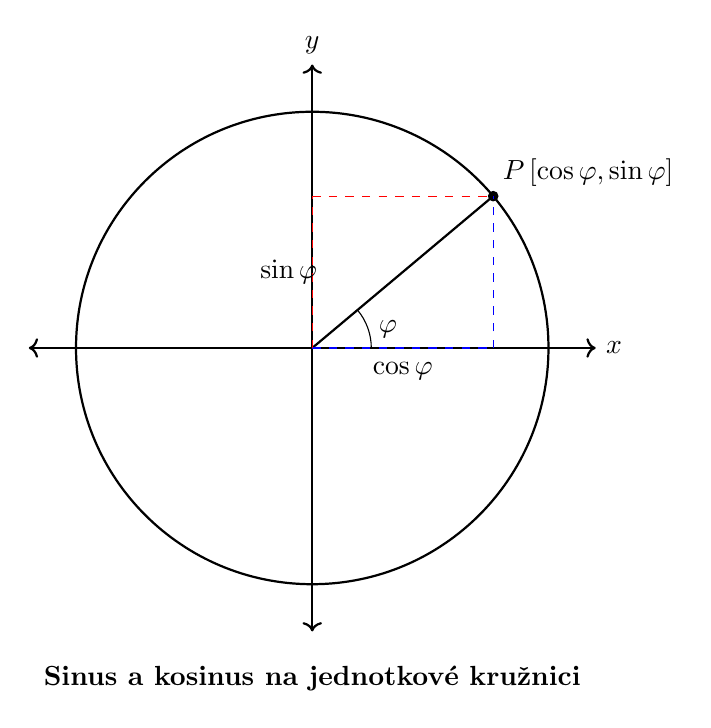
\begin{tikzpicture}[scale=3]
        % === UNIT CIRCLE ===
        \draw[thick] (0,0) circle (1);

        % === AXIS ===
        \draw[<->, thick] (-1.2,0) -- (1.2,0) node[right] {$x$};
        \draw[<->, thick] (0,-1.2) -- (0,1.2) node[above] {$y$};

        % === ANGLE PHI ===
        \draw[thick] (0,0) -- ({cos(40)},{sin(40)});
        \draw (0.25,0) arc (0:40:0.25);
        \node at (0.32,0.08) {$\varphi$};

        % === POINT P ===
        \filldraw[black] ({cos(40)},{sin(40)}) circle (0.02) 
            node[above right] {$P\left[\cos\varphi, \sin\varphi\right]$};
        
        % === COSINE LINE ===
        \draw[dashed,blue] ({cos(40)},0) -- ({cos(40)},{sin(40)});
        \draw[dashed,blue] (0,0) -- ({cos(40)},0);
        \node at ({cos(40)/2},-0.1) {$\cos\varphi$};

        % === SINUS LINE ===
        \draw[dashed,red] (0,{sin(40)}) -- ({cos(40)},{sin(40)});
        \draw[dashed,red] (0,0) -- (0,{sin(40)});
        \node at (-0.1,{sin(40)/2}) {$\sin\varphi$};

        % === TITLE ===
        \node at (0,-1.4) {\textbf{Sinus a kosinus na jednotkové kružnici}};

    \end{tikzpicture}
\end{center}


Z těchto dvou funkcí lze odvodit další dvě, které se často používají při výpočtech v geometrii i v 
analýze. Obě vznikají jako podíl základních funkcí a odpovídají směrnici tečny či směru kolmice v 
konkrétních geometrických konfiguracích.

\begin{notebox}
Pro funkce $\tan\varphi$ a $\cot\varphi$ musíme vždy uvádět definiční obor s vyloučením těch úhlů, 
pro něž by došlo k dělení nulou. To si ukážeme v příslušných definicích níže.
\end{notebox}

Na jednotkové kružnici můžeme definovat tedy i \important{tangens} a \important{kotangens} úhlu $\varphi$ následovně:
\begin{center}
    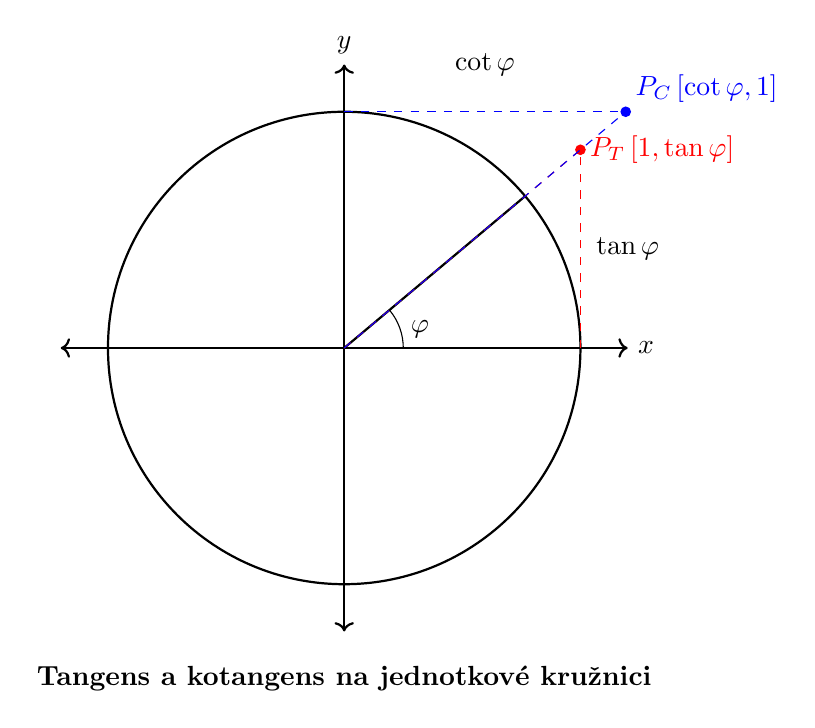
\begin{tikzpicture}[scale=3]
        % === UNIT CIRCLE ===
        \draw[thick] (0,0) circle (1);

        % === AXIS ===
        \draw[<->, thick] (-1.2,0) -- (1.2,0) node[right] {$x$};
        \draw[<->, thick] (0,-1.2) -- (0,1.2) node[above] {$y$};

        % === ANGLE PHI ===
        \draw[thick] (0,0) -- ({cos(40)},{sin(40)});
        \draw (0.25,0) arc (0:40:0.25);
        \node at (0.32,0.08) {$\varphi$};

        % === TANGENS LINE ===
        \draw[dashed,red] (1,0) -- (1,{tan(40)});
        \draw[dashed,red] (0,0) -- (1,{tan(40)});
        \filldraw[red] (1,{tan(40)}) circle (0.02) 
            node[right] {$P_T\left[1,\tan\varphi\right]$};
        \node at (1.2,{tan(40)/2}) {$\tan\varphi$};

        % === KOTANGENS LINE ===
        \draw[dashed,blue] (0,1) -- ({cot(40)},1);
        \draw[dashed,blue] (0,0) -- ({cot(40)},1);
        \filldraw[blue] ({cot(40)},1) circle (0.02) 
            node[above right] {$P_C\left[\cot\varphi,1\right]$};
        \node at ({cot(40)/2},1.2) {$\cot\varphi$};

        % === TITLE ===
        \node at (0,-1.4) {\textbf{Tangens a kotangens na jednotkové kružnici}};

    \end{tikzpicture}
\end{center}

Odboně jako jsme definovali sinus a kosinus, můžeme nyní zavést i definice pro tangens a kotangens:
\begin{definitionbox}
    \textbf{Tangens a kotangens na jednotkové kružnici}\\
    Nechť $P_T[1,\tan\varphi]$ a $P_C[\cot\varphi,1]$ jsou body na přímkách $x=1$ a $y=1$,
    které leží na přímce procházející počátkem a bodem $P[\cos\varphi,\sin\varphi]$. Potom definujeme:
    \[
    \tan\varphi = y_{P_T}, \qquad
    \cot\varphi = x_{P_C},
    \]

    tj. tangens udává svislou souřadnici bodu $P_T$ na přímce $x=1$, zatímco kotangens udává vodorovnou souřadnici bodu $P_C$ na přímce $y=1$.
\end{definitionbox}

\begin{notebox}
    Jednoduše řečeno:
    
    \textbf{sinus} nám říká jaká je vzdálenost mezi bodem na kružnici a osou~$x$,
    
    \textbf{kosinus} jaká je vzdálenost mezi bodem na kružnici a osou~$y$. Tyto vzdálenost mohou být samozřejmě i v záporných hodnotách os $x$ a $y$.
    
    
    A ačkoliv \textbf{tangens} a \textbf{kotangens} nejsou na jednotkové kružnici tak přímočaré jako sinus a kosinus,
    tak je můžeme chápat takéž chápat jako vzdálenost. Nicméně je to vzdálenost, kterou pro \textbf{tangens} udává kolmice vedená z bodu $x=1$ až k průsečíku s přímkou,
    která je vytvořena spojením bodu $P[\cos\varphi,\sin\varphi]$ a počátku souřadnic. A tento průsečík označujeme jako $P_T[1,\tan\varphi]$.

    U \textbf{kotangensu} je to obdobné, jenže kolmice je vedena z bodu $y=1$ a průsečík s přímkou, která je vytvořena spojením bodu $P[\cos\varphi,\sin\varphi]$ 
    a počátku souřadnic, který označujeme jako $P_C[\cot\varphi,1]$.

    A takto definujeme všechny čtyři základní goniometrické funkce na jednotkové kružnici.
\end{notebox}


Nyní tedy můžeme přistoupit k definici jednotlivých goniometrických funkcí a jejich geometrickému 
významu.

% ------------------------------------------
% SINUS
% ------------------------------------------
\subsubsection*{Sinus}

Jak jsme již řekli, \important{sinus} je jednou ze základních goniometrických funkcí, kterou můžeme
na jednotkové kružnici definovat jako svislou souřadnici bodu odpovídajícího danému úhlu.

Sinus je tedy \textbf{periodickou funkcí} s periodou \textbf{$2\pi$} \footnote{protože otočení o $2\pi$ radiánů - $360^\circ$ - nás vrátí zpět na výchozí bod na jednotkové kružnici} 
a její graf odpovídá hladké, pravidelně se střídající vlně, která postupně \textbf{roste}, dosahuje \textbf{maxima}, následně \textbf{klesá}, dosahuje \textbf{minima} a poté opět \textbf{roste}.
Tento fakt opět plyne z geometrické interpretace na jednotkové kružnici, kde se s rostoucím úhlem mění i svislá souřadnice bodu na kružnici.

\begin{center}
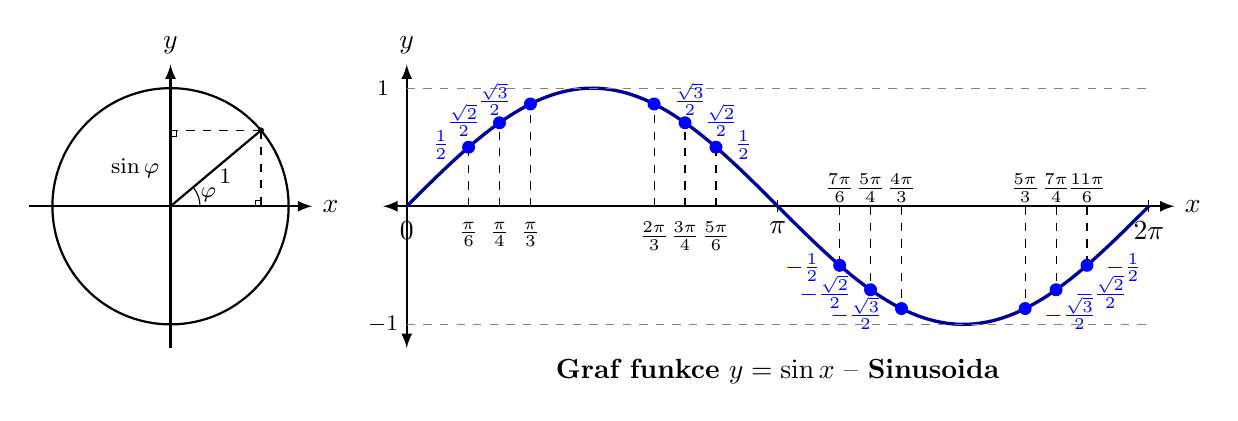
\begin{tikzpicture}[scale=1.5,>=latex]

    % Define angle properly
    \pgfmathsetmacro{\ang}{40}

    % LEFT PART – UNIT CIRCLE
    \begin{scope}[shift={(0,0)}]

        % Axes
        \draw[->, thick] (-1.2,0) -- (1.2,0) node[right] {$x$};
        \draw[->, thick] (0,-1.2) -- (0,1.2) node[above] {$y$};

        % Circle
        \draw[thick] (0,0) circle (1);

        % Angle phi
        \draw[thick] (0,0) -- ({cos(\ang)},{sin(\ang)});
        \draw (0.25,0) arc (0:\ang:0.25);
        \node at (0.32,0.10) {\footnotesize{$\varphi$}};

        % Point on circle
        \filldraw[black] ({cos(\ang)},{sin(\ang)}) circle (0.02);

        % Projections
        \draw[dashed] ({cos(\ang)},{sin(\ang)}) -- ({cos(\ang)},0);
        \draw[dashed] ({cos(\ang)},{sin(\ang)}) -- (0,{sin(\ang)});

        % Right angle markers
        \draw ({cos(\ang)},0) ++(-0.05,0) -- ++(0,0.05) -- ++(0.05,0);
        \draw (0,{sin(\ang)}) ++(0,-0.05) -- ++(0.05,0) -- ++(0,0.05);

        % Labels
        \node at (-0.3,{sin(\ang)/2}) {\footnotesize{$\sin\varphi$}};

        % Radius label
        \node at ({cos(\ang)/2 + 0.08},{sin(\ang)/2 - 0.07}) {\footnotesize{$1$}};

    \end{scope}

    % RIGHT PART – SINE GRAPH
    % RIGHT PART – SINE GRAPH
    \begin{scope}[shift={(2,0)}]

        % Axes
        \draw[<->, thick] (0,-1.2) -- (0,1.2) node[above] {$y$};
        \node at (-0.2,1) {\footnotesize $1$};
        \node at (-0.2,-1) {\footnotesize $-1$};
        \draw[<->, thick] (-0.2,0) -- (6.5,0) node[right] {$x$};

        % Sine curve
        \draw[very thick, blue!60!black, samples=200, domain=0:2*pi]
            plot(\x,{sin(\x r)});

        % π marks
        \foreach \k/\lab in {0/0,1/$\pi$,2/$2\pi$}
        {
            \draw (\k*pi,0.05) -- (\k*pi,-0.05) node[below] {\lab};
        }

        % Horizontal lines ±1
        \draw[dashed, gray] (0,1) -- (2*pi,1);
        \draw[dashed, gray] (0,-1) -- (2*pi,-1);

        % === MARK 30°, 45°, 60° ===

        % 30 degrees (pi/6)
        \pgfmathsetmacro{\xA}{pi/6}
        \pgfmathsetmacro{\yA}{sin(\xA r)}
        \draw[dashed] (\xA,0) -- (\xA,\yA);
        \filldraw[blue] (\xA,\yA) circle (0.05);
        \node[below] at (\xA,-0.05) {\footnotesize $\frac{\pi}{6}$};
        \node[left, blue] at (\xA-0.08,\yA+0.02) {\footnotesize $\frac{1}{2}$};

        % 45 degrees (pi/4)
        \pgfmathsetmacro{\xB}{pi/4}
        \pgfmathsetmacro{\yB}{sin(\xB r)}
        \draw[dashed] (\xB,0) -- (\xB,\yB);
        \filldraw[blue] (\xB,\yB) circle (0.05);
        \node[below] at (\xB,-0.05) {\footnotesize $\frac{\pi}{4}$};
        \node[left, blue] at (\xB-0.08,\yB+0.02) {\footnotesize $\frac{\sqrt{2}}{2}$};

        % 60 degrees (pi/3)
        \pgfmathsetmacro{\xC}{pi/3}
        \pgfmathsetmacro{\yC}{sin(\xC r)}
        \draw[dashed] (\xC,0) -- (\xC,\yC);
        \filldraw[blue] (\xC,\yC) circle (0.05);
        \node[below] at (\xC,-0.05) {\footnotesize $\frac{\pi}{3}$};
        \node[left, blue] at (\xC-0.08,\yC+0.04) {\footnotesize $\frac{\sqrt{3}}{2}$};

        % 120 degrees (2pi/3)
        \pgfmathsetmacro{\xD}{2*pi/3}
        \pgfmathsetmacro{\yD}{sin(\xD r)}
        \draw[dashed] (\xD,0) -- (\xD,\yD);
        \filldraw[blue] (\xD,\yD) circle (0.05);
        \node[below] at (\xD,-0.05) {\footnotesize $\frac{2\pi}{3}$};
        \node[right, blue] at (\xD+0.08,\yD+0.04) {\footnotesize $\frac{\sqrt{3}}{2}$};

        % 135 degrees (3pi/4)
        \pgfmathsetmacro{\xE}{3*pi/4}
        \pgfmathsetmacro{\yE}{sin(\xE r)}
        \draw[dashed] (\xE,0) -- (\xE,\yE);
        \filldraw[blue] (\xE,\yE) circle (0.05);
        \node[below] at (\xE,-0.05) {\footnotesize $\frac{3\pi}{4}$};
        \node[right, blue] at (\xE+0.08,\yE+0.02) {\footnotesize $\frac{\sqrt{2}}{2}$};

        % 150 degrees (5pi/6)
        \pgfmathsetmacro{\xF}{5*pi/6}
        \pgfmathsetmacro{\yF}{sin(\xF r)}
        \draw[dashed] (\xF,0) -- (\xF,\yF);
        \filldraw[blue] (\xF,\yF) circle (0.05);
        \node[below] at (\xF,-0.05) {\footnotesize $\frac{5\pi}{6}$};
        \node[right, blue] at (\xF+0.08,\yF+0.02) {\footnotesize $\frac{1}{2}$};

        % 210 degrees (7pi/6)
        \pgfmathsetmacro{\xG}{7*pi/6}
        \pgfmathsetmacro{\yG}{sin(\xG r)}
        \draw[dashed] (\xG,0) -- (\xG,\yG);
        \filldraw[blue] (\xG,\yG) circle (0.05);
        \node[above] at (\xG,-0.05) {\footnotesize $\frac{7\pi}{6}$};
        \node[left, blue] at (\xG-0.08,\yG-0.02) {\footnotesize $-\frac{1}{2}$};

        % 225 degrees (5pi/4)
        \pgfmathsetmacro{\xH}{5*pi/4}
        \pgfmathsetmacro{\yH}{sin(\xH r)}
        \draw[dashed] (\xH,0) -- (\xH,\yH);
        \filldraw[blue] (\xH,\yH) circle (0.05);
        \node[above] at (\xH,-0.05) {\footnotesize $\frac{5\pi}{4}$};
        \node[left, blue] at (\xH-0.08,\yH-0.02) {\footnotesize $-\frac{\sqrt{2}}{2}$};

        % 240 degrees (4pi/3)
        \pgfmathsetmacro{\xI}{4*pi/3}
        \pgfmathsetmacro{\yI}{sin(\xI r)}
        \draw[dashed] (\xI,0) -- (\xI,\yI);
        \filldraw[blue] (\xI,\yI) circle (0.05);
        \node[above] at (\xI,-0.05) {\footnotesize $\frac{4\pi}{3}$};
        \node[left, blue] at (\xI-0.08,\yI-0.04) {\footnotesize $-\frac{\sqrt{3}}{2}$};

        % 300 degrees (5pi/3)
        \pgfmathsetmacro{\xJ}{5*pi/3}
        \pgfmathsetmacro{\yJ}{sin(\xJ r)}
        \draw[dashed] (\xJ,0) -- (\xJ,\yJ);
        \filldraw[blue] (\xJ,\yJ) circle (0.05);
        \node[above] at (\xJ,-0.05) {\footnotesize $\frac{5\pi}{3}$};
        \node[right, blue] at (\xJ+0.08,\yJ-0.04) {\footnotesize $-\frac{\sqrt{3}}{2}$};

        % 315 degrees (7pi/4)
        \pgfmathsetmacro{\xK}{7*pi/4}
        \pgfmathsetmacro{\yK}{sin(\xK r)}
        \draw[dashed] (\xK,0) -- (\xK,\yK);
        \filldraw[blue] (\xK,\yK) circle (0.05);
        \node[above] at (\xK,-0.05) {\footnotesize $\frac{7\pi}{4}$};
        \node[right, blue] at (\xK+0.08,\yK-0.02) {\footnotesize $-\frac{\sqrt{2}}{2}$};

        % 330 degrees (11pi/6)
        \pgfmathsetmacro{\xL}{11*pi/6}
        \pgfmathsetmacro{\yL}{sin(\xL r)}
        \draw[dashed] (\xL,0) -- (\xL,\yL);
        \filldraw[blue] (\xL,\yL) circle (0.05);
        \node[above] at (\xL,-0.05) {\footnotesize $\frac{11\pi}{6}$};
        \node[right, blue] at (\xL+0.08,\yL-0.02) {\footnotesize $-\frac{1}{2}$};

        % Title
        \node at (3.14,-1.4) {\textbf{Graf funkce} $y=\sin x$ – \textbf{Sinusoida}};

    \end{scope}


\end{tikzpicture}
\end{center}

Sinus však nemusíme definovat jen pomocí jednotkové kružnice. Jako historicky první byla sinusová funkce chápána jako poměr stran v pravoúhlém trojúhelníku.
A přesně tuto definici si nyní připomeneme.

\begin{definitionbox}
Nechť tedy máme pravoúhlý trojúhelník s ostrým úhlem~$\varphi$. Potom definujeme sinus úhlu jako:
\[
\sin\varphi = 
\frac{\textbf{protilehlá odvěsna}}{\textbf{přepona}}
= \frac{a}{c}.
\]

\textbf{Definiční obor:} $\mathbb{R}$, \qquad
\textbf{Obor hodnot:} $\langle -1,1\rangle$, \qquad
\textbf{Perioda:} $2\pi$.
\end{definitionbox}

Tento vztah velmi dobře vystihuje intuitivní představu, že sinus udává, jak „\emph{vysoko}“ úhel směřuje vzhůru.
Při přechodu k jednotkové kružnici se přepona nahradí poloměrem délky~$1$, a právě proto se sinus na
kružnici přirozeně stane svislou souřadnicí bodu, který tomuto úhlu odpovídá.

\begin{center}
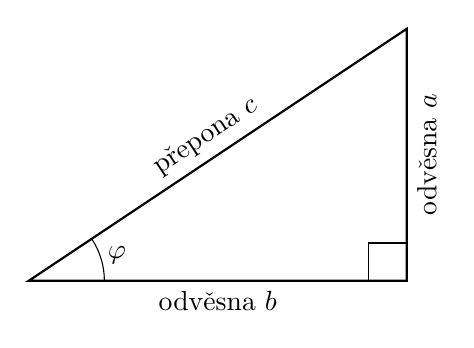
\begin{tikzpicture}[scale=1.6,>=latex]

    % Coordinates of the triangle
    \coordinate (A) at (0,0);        % left bottom (angle φ)
    \coordinate (B) at (3,0);        % right bottom (right angle corner)
    \coordinate (C) at (3,2);        % top vertex

    % Draw triangle
    \draw[thick] 
    (A) -- node[midway,below] {odvěsna $b$} 
    (B) -- node[midway,sloped,below] {odvěsna $a$}
    (C) -- node[midway,sloped,above] {přepona $c$}
    cycle;

    % Angle φ at A
    \draw (0.6,0) arc (0:33:0.6);
    \node at (0.7,0.2) {$\varphi$};

    % Right angle at B
    \draw (B) ++(-0.3,0) -- ++(0,0.3) -- ++(0.3,0);


\end{tikzpicture}
\end{center}


\newpage


% ------------------------------------------
% KOSINUS
% ------------------------------------------
\subsubsection*{Kosinus}

\important{Kosinus} je druhou základní goniometrickou funkcí, kterou na jednotkové kružnici definujeme jako
vodorovnou souřadnici bodu odpovídajícího danému úhlu. 
Stejně jako sinus je i kosinus \textbf{periodickou funkcí} s periodou \textbf{$2\pi$} 
a jeho graf má podobný průběh jako graf sinu, avšak je \textbf{fázově posunutý} o $\frac{\pi}{2}$ radiánů (neboli $90^\circ$).

\begin{center}
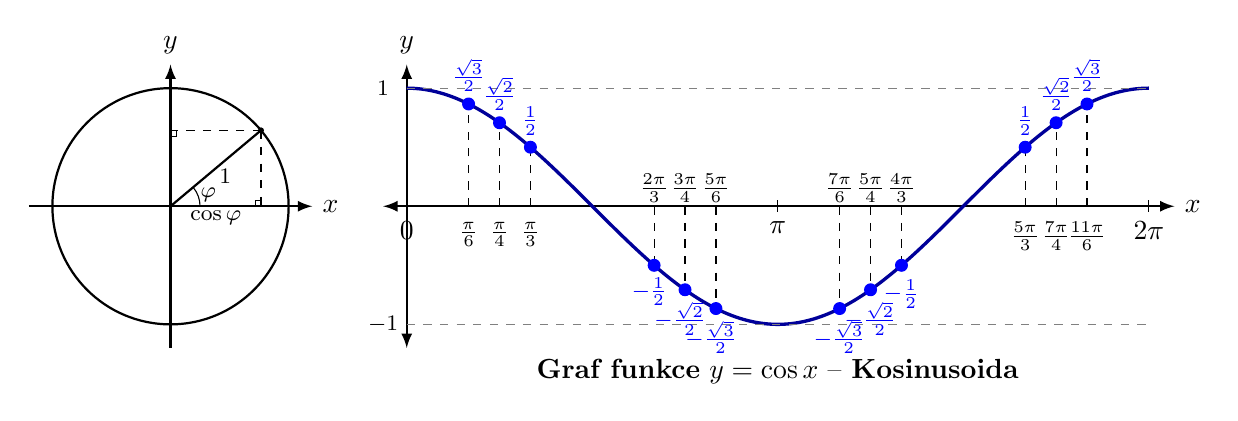
\begin{tikzpicture}[scale=1.5,>=latex]
    % Define angle properly
    \pgfmathsetmacro{\ang}{40}

    % LEFT PART – UNIT CIRCLE
    \begin{scope}[shift={(0,0)}]

        % Axes
        \draw[->, thick] (-1.2,0) -- (1.2,0) node[right] {$x$};
        \draw[->, thick] (0,-1.2) -- (0,1.2) node[above] {$y$};

        % Circle
        \draw[thick] (0,0) circle (1);

        % Angle phi
        \draw[thick] (0,0) -- ({cos(\ang)},{sin(\ang)});
        \draw (0.25,0) arc (0:\ang:0.25);
        \node at (0.32,0.10) {\footnotesize{$\varphi$}};

        % Point on circle
        \filldraw[black] ({cos(\ang)},{sin(\ang)}) circle (0.02);

        % Projections
        \draw[dashed] ({cos(\ang)},{sin(\ang)}) -- ({cos(\ang)},0);
        \draw[dashed] ({cos(\ang)},{sin(\ang)}) -- (0,{sin(\ang)});

        % Right angle markers
        \draw ({cos(\ang)},0) ++(-0.05,0) -- ++(0,0.05) -- ++(0.05,0);
        \draw (0,{sin(\ang)}) ++(0,-0.05) -- ++(0.05,0) -- ++(0,0.05);

        % Labels
        \node at ({cos(\ang)/2},-0.1) {\footnotesize{$\cos\varphi$}};

        % Radius label
        \node at ({cos(\ang)/2 + 0.08},{sin(\ang)/2 - 0.07}) {\footnotesize{$1$}};

    \end{scope}

    % RIGHT PART – COSINE GRAPH
    \begin{scope}[shift={(2,0)}]

        % Axes
        \draw[<->, thick] (0,-1.2) -- (0,1.2) node[above] {$y$};
        \node at (-0.2,1) {\footnotesize $1$};

        \node at (-0.2,-1) {\footnotesize $-1$};
        \draw[<->, thick] (-0.2,0) -- (6.5,0) node[right] {$x$};

        % Cosine curve
        \draw[very thick, blue!60!black, samples=200, domain=0:2*pi]
            plot(\x,{cos(\x r)});

        % π marks
        \foreach \k/\lab in {0/0,1/$\pi$,2/$2\pi$}
        {
            \draw (\k*pi,0.05) -- (\k*pi,-0.05) node[below] {\lab};
        }

        % Horizontal lines ±1
        \draw[dashed, gray] (0,1) -- (2*pi,1);
        \draw[dashed, gray] (0,-1) -- (2*pi,-1);

        % === MARK 30°, 45°, 60°, 120°, 135°, 150°, 180°, 210°, 240°, 300°, 315°, 330° ===

        % 30 degrees (pi/6)
        \pgfmathsetmacro{\xB}{pi/6}
        \pgfmathsetmacro{\yB}{cos(\xB r)}
        \draw[dashed] (\xB,0) -- (\xB,\yB);
        \filldraw[blue] (\xB,\yB) circle (0.05);
        \node[below] at (\xB,-0.05) {\footnotesize $\frac{\pi}{6}$};
        \node[above, blue] at (\xB,\yB+0.02) {\footnotesize $\frac{\sqrt{3}}{2}$};

        % 45 degrees (pi/4)
        \pgfmathsetmacro{\xC}{pi/4}
        \pgfmathsetmacro{\yC}{cos(\xC r)}
        \draw[dashed] (\xC,0) -- (\xC,\yC);
        \filldraw[blue] (\xC,\yC) circle (0.05);
        \node[below] at (\xC,-0.05) {\footnotesize $\frac{\pi}{4}$};
        \node[above, blue] at (\xC,\yC+0.02) {\footnotesize $\frac{\sqrt{2}}{2}$};

        % 60 degrees (pi/3)
        \pgfmathsetmacro{\xD}{pi/3}
        \pgfmathsetmacro{\yD}{cos(\xD r)}
        \draw[dashed] (\xD,0) -- (\xD,\yD);
        \filldraw[blue] (\xD,\yD) circle (0.05);
        \node[below] at (\xD,-0.05) {\footnotesize $\frac{\pi}{3}$};
        \node[above, blue] at (\xD,\yD+0.02) {\footnotesize $\frac{1}{2}$};

        % 120 degrees (2pi/3)
        \pgfmathsetmacro{\xF}{2*pi/3}
        \pgfmathsetmacro{\yF}{cos(\xF r)}
        \draw[dashed] (\xF,0) -- (\xF,\yF);
        \filldraw[blue] (\xF,\yF) circle (0.05);
        \node[above] at (\xF,-0.05) {\footnotesize $\frac{2\pi}{3}$};
        \node[below, blue] at (\xF-0.04,\yF-0.02) {\footnotesize $-\frac{1}{2}$};

        % 135 degrees (3pi/4)
        \pgfmathsetmacro{\xG}{3*pi/4}
        \pgfmathsetmacro{\yG}{cos(\xG r)}
        \draw[dashed] (\xG,0) -- (\xG,\yG);
        \filldraw[blue] (\xG,\yG) circle (0.05);
        \node[above] at (\xG,-0.05) {\footnotesize $\frac{3\pi}{4}$};
        \node[below, blue] at (\xG-0.04,\yG-0.02) {\footnotesize $-\frac{\sqrt{2}}{2}$};

        % 150 degrees (5pi/6)
        \pgfmathsetmacro{\xH}{5*pi/6}
        \pgfmathsetmacro{\yH}{cos(\xH r)}
        \draw[dashed] (\xH,0) -- (\xH,\yH);
        \filldraw[blue] (\xH,\yH) circle (0.05);
        \node[above] at (\xH,-0.05) {\footnotesize $\frac{5\pi}{6}$};
        \node[below, blue] at (\xH-0.04,\yH-0.02) {\footnotesize $-\frac{\sqrt{3}}{2}$};

        % 210 degrees (7pi/6)
        \pgfmathsetmacro{\xJ}{7*pi/6}
        \pgfmathsetmacro{\yJ}{cos(\xJ r)}
        \draw[dashed] (\xJ,0) -- (\xJ,\yJ);
        \filldraw[blue] (\xJ,\yJ) circle (0.05);
        \node[above] at (\xJ,-0.05) {\footnotesize $\frac{7\pi}{6}$};
        \node[below, blue] at (\xJ,\yJ-0.02) {\footnotesize $-\frac{\sqrt{3}}{2}$};

        % 225 degrees (5pi/4)
        \pgfmathsetmacro{\xK}{5*pi/4}
        \pgfmathsetmacro{\yK}{cos(\xK r)}
        \draw[dashed] (\xK,0) -- (\xK,\yK);
        \filldraw[blue] (\xK,\yK) circle (0.05);
        \node[above] at (\xK,-0.05) {\footnotesize $\frac{5\pi}{4}$};
        \node[below, blue] at (\xK,\yK-0.02) {\footnotesize $-\frac{\sqrt{2}}{2}$};

        % 240 degrees (4pi/3)
        \pgfmathsetmacro{\xL}{4*pi/3}
        \pgfmathsetmacro{\yL}{cos(\xL r)}
        \draw[dashed] (\xL,0) -- (\xL,\yL);
        \filldraw[blue] (\xL,\yL) circle (0.05);
        \node[above] at (\xL,-0.05) {\footnotesize $\frac{4\pi}{3}$};
        \node[below, blue] at (\xL,\yL-0.04) {\footnotesize $-\frac{1}{2}$};

        % 300 degrees (5pi/3)
        \pgfmathsetmacro{\xM}{5*pi/3}
        \pgfmathsetmacro{\yM}{cos(\xM r)}
        \draw[dashed] (\xM,0) -- (\xM,\yM);
        \filldraw[blue] (\xM,\yM) circle (0.05);
        \node[below] at (\xM,-0.05) {\footnotesize $\frac{5\pi}{3}$};
        \node[above, blue] at (\xM,\yM+0.02) {\footnotesize $\frac{1}{2}$};

        % 315 degrees (7pi/4)
        \pgfmathsetmacro{\xN}{7*pi/4}
        \pgfmathsetmacro{\yN}{cos(\xN r)}
        \draw[dashed] (\xN,0) -- (\xN,\yN);
        \filldraw[blue] (\xN,\yN) circle (0.05);
        \node[below] at (\xN,-0.05) {\footnotesize $\frac{7\pi}{4}$};
        \node[above, blue] at (\xN,\yN+0.02) {\footnotesize $\frac{\sqrt{2}}{2}$};

        % 330 degrees (11pi/6)
        \pgfmathsetmacro{\xO}{11*pi/6}
        \pgfmathsetmacro{\yO}{cos(\xO r)}
        \draw[dashed] (\xO,0) -- (\xO,\yO);
        \filldraw[blue] (\xO,\yO) circle (0.05);
        \node[below] at (\xO,-0.05) {\footnotesize $\frac{11\pi}{6}$};
        \node[above, blue] at (\xO,\yO+0.02) {\footnotesize $\frac{\sqrt{3}}{2}$};

        % Title
        \node at (3.14,-1.4) {\textbf{Graf funkce} $y=\cos x$ – \textbf{Kosinusoida}};

    \end{scope}
\end{tikzpicture}
\end{center}

\textbf{Kosinus} můžeme také definovat, stejně jako \emph{sinus} pomocí pravoúhlého trojúhelníku, 
kde představuje poměr délky přilehlé odvěsny k délce přepony.

\begin{definitionbox}
Nechť tedy máme pravoúhlý trojúhelník s ostrým úhlem~$\varphi$. Potom definujeme kosinus úhlu jako:
\[
\cos\varphi = 
\frac{\textbf{přilehlá odvěsna}}{\textbf{přepona}}
= \frac{b}{c}.
\]
\textbf{Definiční obor:} $\mathbb{R}$, \qquad
\textbf{Obor hodnot:} $\langle -1,1\rangle$, \qquad
\textbf{Perioda:} $2\pi$.
\end{definitionbox}

Tento vztah opět velmi dobře vystihuje intuitivní představu, že kosinus udává, jak „\emph{dál}“ úhel směřuje doprava.
Při přechodu k jednotkové kružnici se přepona nahradí poloměrem délky~$1$, a právě proto se kosinus na
kružnici přirozeně stane vodorovnou souřadnicí bodu, který tomuto úhlu odpovídá.

\begin{center}
    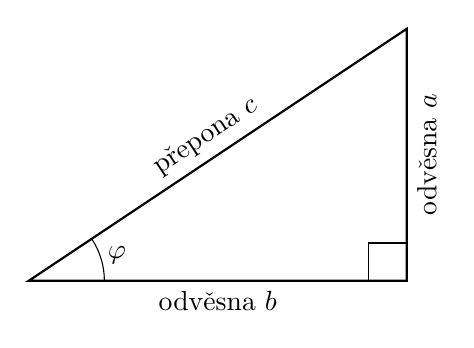
\begin{tikzpicture}[scale=1.6,>=latex]
        
        % Coordinates of the triangle
        \coordinate (A) at (0,0);        % left bottom (angle φ)
        \coordinate (B) at (3,0);        % right bottom (right angle corner)
        \coordinate (C) at (3,2);        % top vertex

        % Draw triangle
        \draw[thick] 
        (A) -- node[midway,below] {odvěsna $b$} 
        (B) -- node[midway,sloped,below] {odvěsna $a$}
        (C) -- node[midway,sloped,above] {přepona $c$}
        cycle;

        % Angle φ at A
        \draw (0.6,0) arc (0:33:0.6);
        \node at (0.7,0.2) {$\varphi$};

        % Right angle at B
        \draw (B) ++(-0.3,0) -- ++(0,0.3) -- ++(0.3,0);

    \end{tikzpicture}
\end{center}


\newpage



% ------------------------------------------
% TANGENS
% ------------------------------------------
\subsubsection*{Tangens}

\important{Tangens} úhlu~$\varphi$ vzniká jako \textbf{podíl hodnot sinu a kosinu},
což znamená, že popisuje \textbf{strmost} neboli \textbf{směrnici}
\footnote{O směrnici jsme již slyšeli během lineárních funkcí, kde u přepdpisu $y=ax+b$ byla směrnice rovna koeficientu $a$, která nám říkala přesně to, jak moc je přímka strmá.} 
příslušného směru na jednotkové 
kružnici. Funkce není definována v úhlech, kde je kosinus roven nule, tedy 
\[
\varphi = \frac{\pi}{2} + k\pi,\qquad k\in\mathbb{Z},
\]
protože v takových bodech bychom dělili nulou. Tyto hodnoty, kde bychom dělili nulou, jsou
\textbf{vertikální asymptoty} funkce tangens. Tangens tedy nabývá všech reálných hodnot až na tyto body
a jeho perioda je $\pi$.




\begin{definitionbox}
    \[
    \tan\varphi = \frac{\sin\varphi}{\cos\varphi},
    \qquad \varphi \neq \frac{\pi}{2} + k\pi.
    \]

    \textbf{Definiční obor:} $\mathbb{R} \setminus \left\{\frac{\pi}{2} + k\pi; k\in\mathbb{Z}\right\}$, \qquad
    \textbf{Obor hodnot:} $\mathbb{R}$, \qquad
    \textbf{Perioda:} $\pi$.
\end{definitionbox}

\begin{center}
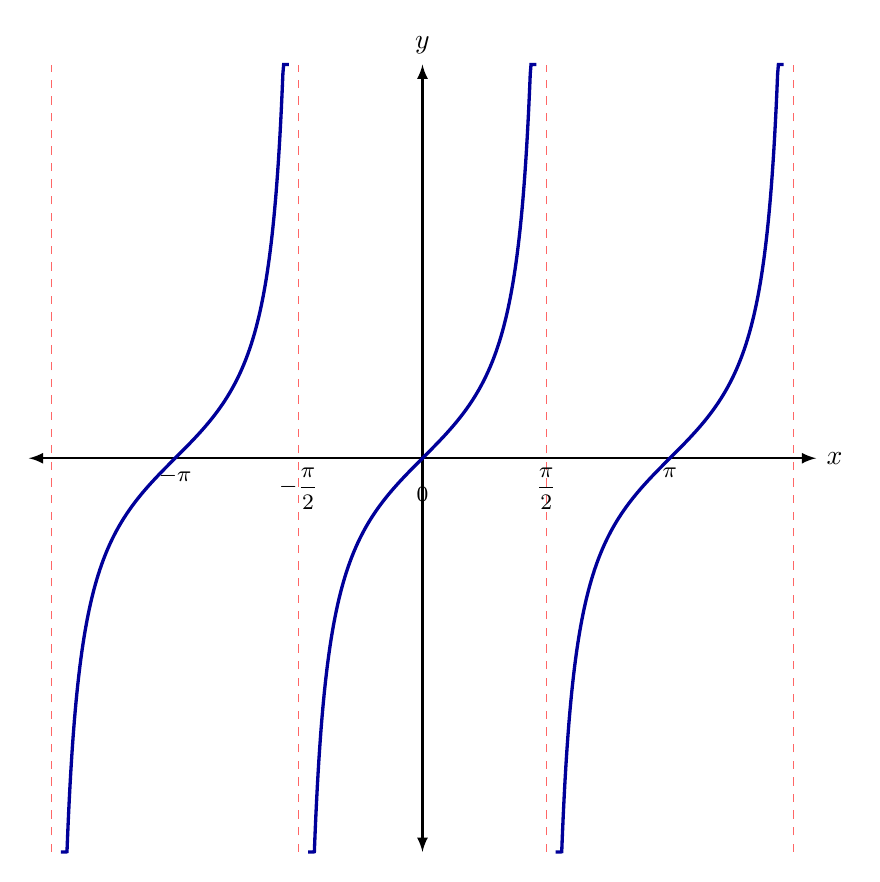
\begin{tikzpicture}[scale=1, >=latex]

% ==== AXES ====
\draw[<->, thick] (-5,0) -- (5,0) node[right] {$x$};
\draw[<->, thick] (0,-5) -- (0,5) node[above] {$y$};

% ==== VERTICAL ASYMPTOTES ====
\foreach \k in {-3,-1,1,3}{
    \draw[dashed, red!60] ({\k*pi/2}, -5) -- ({\k*pi/2}, 5);
}

% ==== TANGENT CURVES (bounded to ±5) ====
\draw[very thick, blue!60!black, samples=300, domain=-3*pi/2+0.12:-pi/2-0.12]
    plot(\x,{min(max(tan(\x r), -5), 5)});

\draw[very thick, blue!60!black, samples=300, domain=-pi/2+0.12:pi/2-0.12]
    plot(\x,{min(max(tan(\x r), -5), 5)});

\draw[very thick, blue!60!black, samples=300, domain=pi/2+0.12:3*pi/2-0.12]
    plot(\x,{min(max(tan(\x r), -5), 5)});



\node[below] at (0,-0.25) {\footnotesize $0$};
\node[below] at ({-pi},0) {\footnotesize $-\pi$};
\node[below] at ({-pi/2},0) {\footnotesize $-\dfrac{\pi}{2}$};
\node[below] at ({pi},0) {\footnotesize $\pi$};
\node[below] at ({pi/2},0) {\footnotesize $\dfrac{\pi}{2}$};


\end{tikzpicture}
\end{center}

Tangens lze také interpretovat geometricky jako \textbf{směrnici} přímky, která prochází počátkem
a bodem na jednotkové kružnici odpovídajícím úhlu~$\varphi$. Tato interpretace opět velmi dobře vystihuje
to, proč tangens nabývá všech reálných hodnot – směrnice přímky může být libovolně velká či malá.
Navíc je zřejmé, proč tangens není definován v úhlech, kde je kosinus nulový – v těchto bodech je přímka
svislá a směrnice tak není definována.



\newpage



% ------------------------------------------
% COTANGENS
% ------------------------------------------
\subsubsection*{Kotangens}

\important{Kotangens} úhlu~$\varphi$ vzniká jako \textbf{inverzní hodnota tangensu}, tedy jako
\textbf{podíl kosinu a sinu}. Funkce není definována v úhlech, kde je sinus roven nule, tedy
\[
\varphi = k\pi,\qquad k\in\mathbb{Z},
\]
protože v takových bodech bychom dělili nulou. Tyto hodnoty, kde bychom dělili nulou, jsou
\textbf{vertikální asymptoty} funkce kotangens. Kotangens tedy nabývá všech reálných hodnot až na tyto body
a jeho perioda je $\pi$.

\begin{definitionbox}
    \[
    \cot\varphi = \frac{\cos\varphi}{\sin\varphi},
    \qquad \varphi \neq k\pi.
    \]

    \textbf{Definiční obor:} $\mathbb{R} \setminus \left\{k\pi; k\in\mathbb{Z}\right\}$, \qquad
    \textbf{Obor hodnot:} $\mathbb{R}$, \qquad
    \textbf{Perioda:} $\pi$.
\end{definitionbox}

\begin{center}
    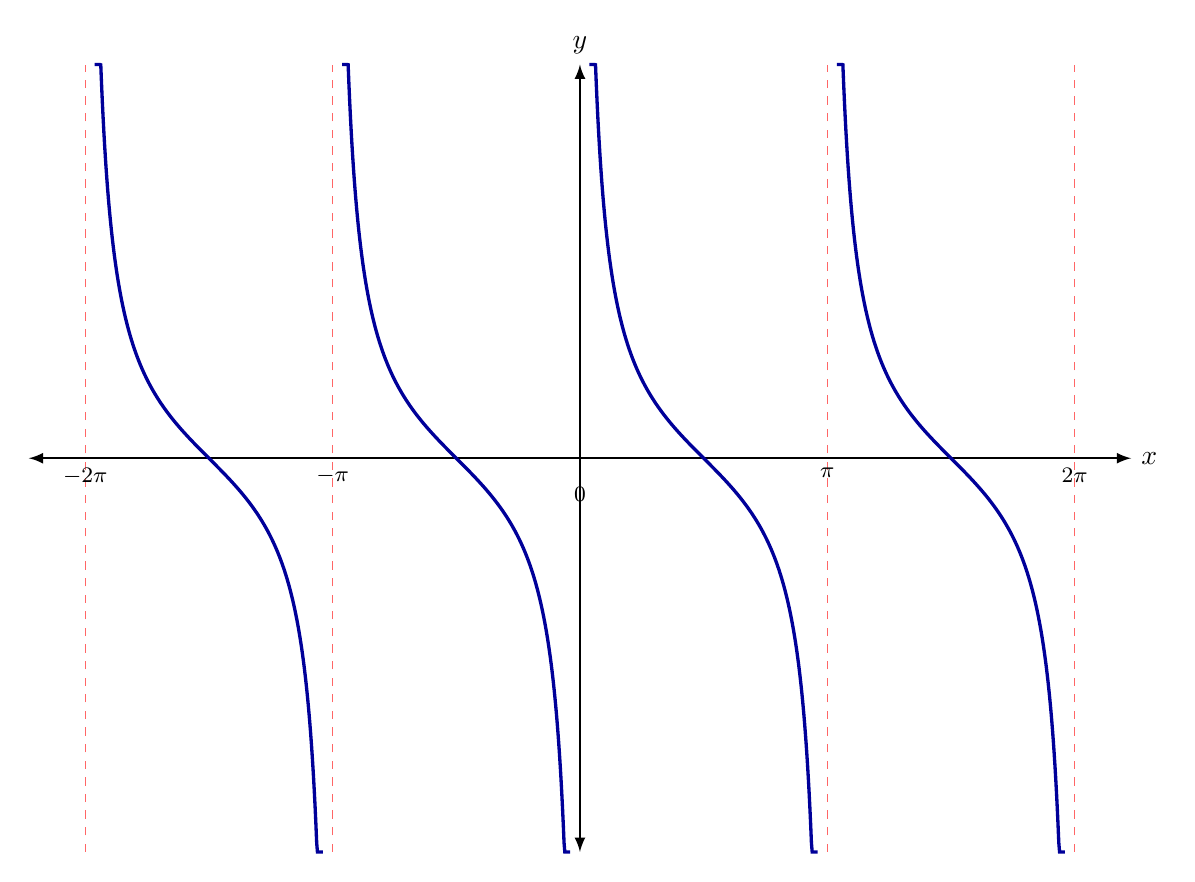
\begin{tikzpicture}[scale=1, >=latex]
        % ==== AXES ====
        \draw[<->, thick] (-7,0) -- (7,0) node[right] {$x$};
        \draw[<->, thick] (0,-5) -- (0,5) node[above] {$y$};
        
        % ==== VERTICAL ASYMPTOTES ====
        \foreach \k in {-2,-1,1,2}{
            \draw[dashed, red!60] ({\k*pi}, -5) -- ({\k*pi}, 5);
        }
        
        % ==== COTANGENT CURVES (bounded to ±5) ====
        \draw[very thick, blue!60!black, samples=300, domain=-2*pi+0.12:-pi-0.12]
            plot(\x,{min(max(cot(\x r), -5), 5)});
        \draw[very thick, blue!60!black, samples=300, domain=-pi+0.12:0-0.12]
            plot(\x,{min(max(cot(\x r), -5), 5)});
        \draw[very thick, blue!60!black, samples=300, domain=0+0.12:pi-0.12]
            plot(\x,{min(max(cot(\x r), -5), 5)});
        \draw[very thick, blue!60!black, samples=300, domain=pi+0.12:2*pi-0.12]
            plot(\x,{min(max(cot(\x r), -5), 5)});

        % === LABELS ===
        \node[below] at (0,-0.25) {\footnotesize $0$};
        \node[below] at ({-pi},0) {\footnotesize $-\pi$};
        \node[below] at ({pi},0) {\footnotesize $\pi$};
        \node[below] at ({-2*pi},0) {\footnotesize $-2\pi$};
        \node[below] at ({2*pi},0) {\footnotesize $2\pi$};


    \end{tikzpicture}
\end{center}

Kotangens lze také interpretovat geometricky jako \textbf{inverzní směrnici} přímky, která prochází počátkem
a bodem na jednotkové kružnici odpovídajícím úhlu~$\varphi$. Tato interpretace opět velmi dobře vystihuje
to, proč kotangens nabývá všech reálných hodnot – inverzní směrnice přímky může být libovolně velká či malá.
Navíc je zřejmé, proč kotangens není definován v úhlech, kde je sinus nulový – v těchto bodech je přímka
vodorovná a inverzní směrnice tak není definována.



\newpage


\section{Tabulkové hodnoty goniometrických funkcí}

V této části odvodíme tabulkové hodnoty goniometrických funkcí pro úhly $30^\circ$, $45^\circ$, $60^\circ$ a $90^\circ$.
Tyto hodnoty jsou často využívány a je dobré je znát zpaměti.

Při jejich odvozování využijeme faktu, že goniometrické funkce lze definovat pomocí pravoúhlého trojúhelníku.

\bigskip
\textbf{Hodnoty pro $0^\circ$, $45^\circ$ a $90^\circ$:}

Nejprve si připomeneme vlastnosti pravoúhlého trojúhelníku s úhly $45^\circ$, $45^\circ$ a $90^\circ$. 
Rovnoramenný pravoúhlý trojúhelník s úhly $45^\circ$, $45^\circ$ a $90^\circ$ má dvě shodné odvěsny $a$ a $b$ 
a přeponu můžeme vyjádřit pomocí Pythagorovy věty:
\[
c^2 = a^2 + b^2,
\]
protože odvěsny jsou shodné, můžeme nahradit $b$ za $a$:
\[
c^2 = a^2 + a^2,
\]
odkud plyne délka přepony:
\[
c = \sqrt{a^2 + a^2} = \sqrt{2a^2} = a\sqrt{2}.
\]

\begin{center}
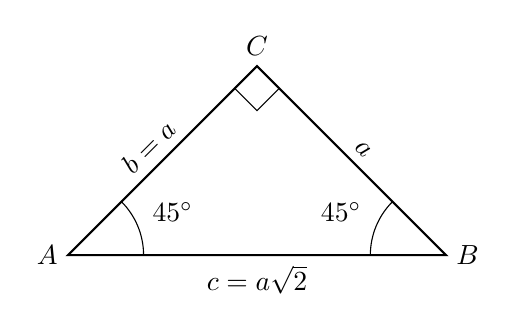
\begin{tikzpicture}[
    scale=1.6,
    >=latex
]


    % Coordinates
    \coordinate (A) at (0,0);      % left bottom
    \coordinate (B) at (3,0);      % right bottom
    \coordinate (C) at (1.5,1.5);  % top (right angle)

    % Draw triangle
    \draw[thick] (0,0) coordinate[label=left:$A$] (A)
    -- node[midway,below] {$c=a\sqrt{2}$} 
    (3,0) coordinate[label=right:$B$] (B)
    -- node[midway,sloped,above] {$a$} 
    (1.5,1.5) coordinate[label=above:$C$] (C)
    -- node[midway,sloped,above] {$b=a$}
    cycle;

    \tkzMarkRightAngle(A,C,B);
    % Angle at A – 45°
    \tkzMarkAngle[size=0.6](B,A,C)
    \tkzLabelAngle[pos=0.9](B,A,C){$45^\circ$}

    % Angle at B – 45°
    \tkzMarkAngle[size=0.6](C,B,A)
    \tkzLabelAngle[pos=0.9](C,B,A){$45^\circ$}

\end{tikzpicture}
\end{center}


Pomocí definic goniometrických funkcí v pravoúhlém trojúhelníku nyní snadno odvodíme tabulkové hodnoty.

% ------------------------------------------
% ÚHEL 45
% ------------------------------------------
\subsubsection*{Hodnoty pro $\boldsymbol{45^\circ}$}

\paragraph{Sinus}
\[
\sin 45^\circ = \frac{\text{protilehlá odvěsna}}{\text{přepona}}
= \frac{a}{a\sqrt{2}}
= \frac{1}{\sqrt{2}}
= \frac{\sqrt{2}}{2}.
\]

\paragraph{Kosinus}
\[
\cos 45^\circ = \frac{\text{přilehlá odvěsna}}{\text{přepona}}
= \frac{a}{a\sqrt{2}}
= \frac{1}{\sqrt{2}}
= \frac{\sqrt{2}}{2}.
\]

\paragraph{Tangens}
\[
\tan 45^\circ
= \frac{\sin 45^\circ}{\cos 45^\circ}
= \frac{\frac{\sqrt{2}}{2}}{\frac{\sqrt{2}}{2}}
= 1.
\]

\paragraph{Cotangens}
\[
\cot 45^\circ
= \frac{\cos 45^\circ}{\sin 45^\circ}
= \frac{\frac{\sqrt{2}}{2}}{\frac{\sqrt{2}}{2}}
= 1.
\]

% ------------------------------------------
% ÚHEL 90
% ------------------------------------------
\subsubsection*{Hodnoty pro $\boldsymbol{90^\circ}$}

Hodnoty goniometrických funkcí pro úhel $90^\circ$ nelze odvodit pomocí pravoúhlého trojúhelníku,
protože ač existuje trojúhelník s úhlem $90^\circ$. 
Tak neexistuje pravoúhlý trojúhelník s dalším úhlem, který má $90^\circ$. V ten moment by totiž součet úhlů v trojúhelníku byl větší než $180^\circ$.
Proto využijeme definice goniometrických funkcí na jednotkové kružnici.

\paragraph{Sinus}
\[\sin 90^\circ = 1,\]
protože na jednotkové kružnici je pro úhel $90^\circ$ hodnota $y$ rovna $1$.

\paragraph{Kosinus}
\[\cos 90^\circ = 0,\]
protože na jednotkové kružnici je pro úhel $90^\circ$ hodnota $x$ rovna $0$.

\paragraph{Tangens}
\[
\tan 90^\circ
= \frac{\sin 90^\circ}{\cos 90^\circ}
= \frac{1}{0},
\]
protože bychom dělili nulou, je tangens nedefinován.

\paragraph{Cotangens}
\[
\cot 90^\circ
= \frac{\cos 90^\circ}{\sin 90^\circ}
= \frac{0}{1} = 0.
\]

% ------------------------------------------
% ÚHEL 0
% ------------------------------------------

\subsubsection*{Hodnoty pro $\boldsymbol{0^\circ}$}
Stejně jako u úhlu $90^\circ$ nelze hodnoty goniometrických funkcí pro úhel $0^\circ$ odvodit pomocí pravoúhlého trojúhelníku.
Proto využijeme opět definice goniometrických funkcí na jednotkové kružnici.

\paragraph{Sinus}
\[\sin 0^\circ = 0,\]
protože na jednotkové kružnici je pro úhel $0^\circ$ hodnota $y$ rovna $0$.

\paragraph{Kosinus}
\[\cos 0^\circ = 1,\]
protože na jednotkové kružnici je pro úhel $0^\circ$ hodnota $x$ rovna $1$.

\paragraph{Tangens}
\[
\tan 0^\circ
= \frac{\sin 0^\circ}{\cos 0^\circ}
= \frac{0}{1} = 0.
\]

\paragraph{Cotangens}
\[
\cot 0^\circ
= \frac{\cos 0^\circ}{\sin 0^\circ}
= \frac{1}{0},
\]
protože bychom dělili nulou, je kotangens nedefinován.



\bigskip
\textbf{Hodnoty pro $30^\circ$ a $60^\circ$:}

A nyní odvodíme hodnoty goniometrických funkcí pro úhel $30^\circ$ a $60^\circ$.
Nejprve bude potřeba si znázornit trojúhelník který má úhly $30^\circ$, $60^\circ$ a $90^\circ$.
Takový trojúhelník lze získat z rovnostranného trojúhelníku, který má všechny úhly rovny $60^\circ$.

Pokud do rovnostranného trojúhelníku s délkou stran $a$ narýsujeme výšku $v$, rozdělíme tím rovnostranný trojúhelník 
na dva shodné pravoúhlé trojúhelníky s úhly $30^\circ$, $60^\circ$ a $90^\circ$. 

\begin{center}
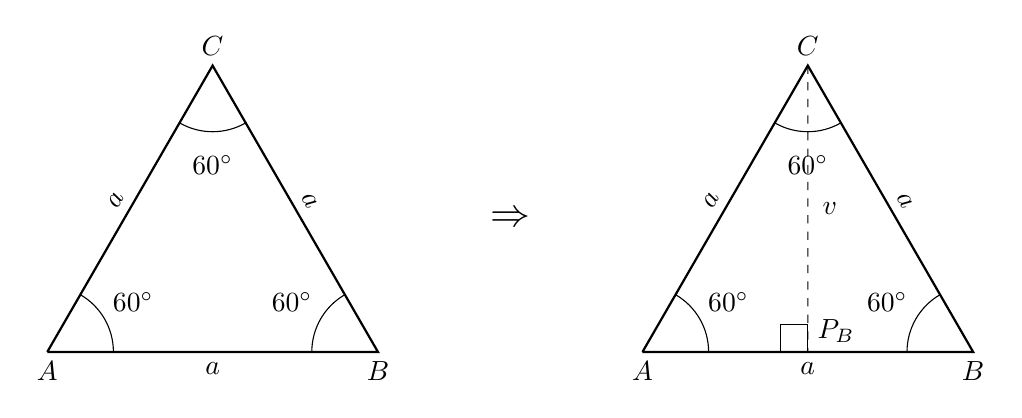
\begin{tikzpicture}[scale=1.4,>=latex]

% ============================================
% LEFT SIDE – EQUILATERAL TRIANGLE
% ============================================
        % Coordinates
        \coordinate (A) at (0,0);
        \coordinate (B) at (3,0);
        \coordinate (C) at (1.5,2.598); % height = a*sqrt(3)/2, here scaled
        % Triangle
        \draw[thick] (A) -- node[midway,below] {$a$} (B)
                      -- node[midway,sloped,above] {$a$} (C)
                      -- node[midway,sloped,above] {$a$} (A);
        % Angle labels              
        \tkzMarkAngle [size=0.6](B,A,C)
        \tkzLabelAngle [pos=0.9](B,A,C){$60^\circ$}
        \tkzMarkAngle [size=0.6](C,B,A)
        \tkzLabelAngle [pos=0.9](C,B,A){$60^\circ$}
        \tkzMarkAngle [size=0.6](A,C,B)
        \tkzLabelAngle [pos=0.9](A,C,B){$60^\circ$}
        % Bottom labels
        \node at (A) [below] {$A$};
        \node at (B) [below] {$B$};
        \node at (C) [above] {$C$};

% ============================================
% Arrow between triangles
% ============================================

\node at (4.2,1.2) {\Large $\Rightarrow$};

% ============================================
% RIGHT SIDE –  TRIANGLE WITH v
% ============================================
        % Coordinates
        \coordinate (A) at (0 + 5.4,0);
        \coordinate (B) at (3 + 5.4,0);
        \coordinate (C) at (1.5 + 5.4,2.598); % height = a*sqrt(3)/2, here scaled
        \coordinate (P_B) at (1.5 + 5.4,0); % foot of the height from C
        % Triangle
        \draw[thick] (A) -- node[midway,below] {$a$} (B)
                      -- node[midway,sloped,above] {$a$} (C)
                      -- node[midway,sloped,above] {$a$} (A);
        
        % Angle labels
        \tkzMarkAngle [size=0.6](B,A,C)
        \tkzLabelAngle [pos=0.9](B,A,C){$60^\circ$}
        \tkzMarkAngle [size=0.6](C,B,A)
        \tkzLabelAngle [pos=0.9](C,B,A){$60^\circ$}
        \tkzMarkAngle [size=0.6](A,C,B)
        \tkzLabelAngle [pos=0.9](A,C,B){$60^\circ$}
        \tkzMarkRightAngle (A,P_B,C);
        % Bottom labels
        \node at (A) [below] {$A$};
        \node at (B) [below] {$B$};
        \node at (C) [above] {$C$};
        \node at (P_B) [above right] {$P_B$};
        % Height (dashed)
        \draw[dashed] (C) -- (1.5 + 5.4,0);
        % Height label
        \node at (1.5 + 5.4 + 0.2,1.3) {$v$};
\end{tikzpicture}
\end{center}



K určení úhlů v tomto pravoúhlém trojúhelníku však musíme znát ještě délku výšky rovnostranného trojúhelníku.
Anebo ji alespoň vyjádřit pomocí délky strany $a$.

\bigskip
Prvně tedy odvodíme proč výška v rovnostrnném trojúhelníku $v$ je rovna $a\frac{\sqrt{3}}{2}$.
Použijeme Pythagorovu větu v pravoúhlém trojúhelníku $AP_BC$, kde $P_B$ je půlka strany $AB$, tedy $P_B$ je patou výšky z vrcholu $C$ na stranu $AB$:
\[c^2 = a^2 + b^2\]
\[AC^2 = AP_B^2 + CP_B^2,\]
\[a^2 = \left(\frac{a}{2}\right)^2 + v^2,\]
odkud plyne délka výšky:
\[v = \sqrt{a^2 - \left(\frac{a}{2}\right)^2} = \sqrt{a^2 - \frac{a^2}{4}} = \sqrt{\frac{3a^2}{4}} = a\frac{\sqrt{3}}{2}.\]

\begin{center}
    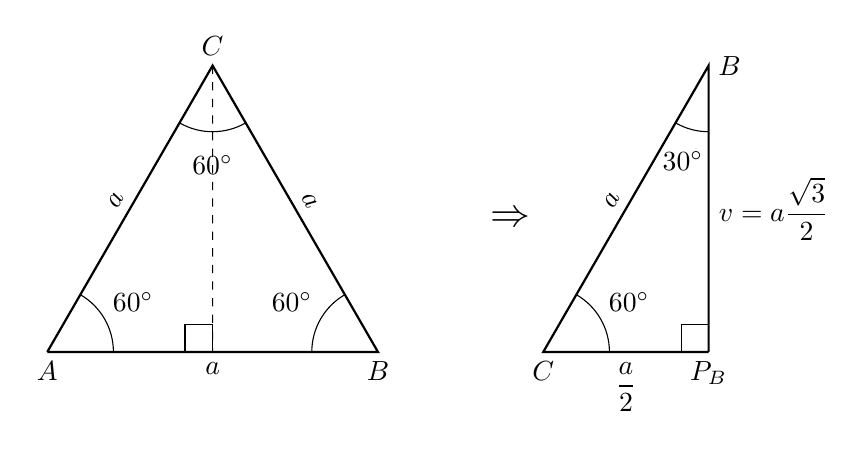
\begin{tikzpicture}[scale=1.4,>=latex]

        % ============================================
        % LEFT SIDE – EQUILATERAL TRIANGLE
        % ============================================

        % Coordinates
        \coordinate (A) at (0,0);
        \coordinate (B) at (3,0);
        \coordinate (C) at (1.5,2.598); % height = a*sqrt(3)/2, here scaled
        \coordinate (P_B) at (1.5,0); % foot of the height from C

        % Triangle
        \draw[thick] (A) -- node[midway,below] {$a$} (B)
                      -- node[midway,sloped,above] {$a$} (C)
                      -- node[midway,sloped,above] {$a$} (A);

        % Angle labels              
        \tkzMarkAngle [size=0.6](B,A,C)
        \tkzLabelAngle [pos=0.9](B,A,C){$60^\circ$}
        \tkzMarkAngle [size=0.6](C,B,A)
        \tkzLabelAngle [pos=0.9](C,B,A){$60^\circ$}
        \tkzMarkAngle [size=0.6](A,C,B)
        \tkzLabelAngle [pos=0.9](A,C,B){$60^\circ$}
        \tkzMarkRightAngle (A,P_B,C);

        % Bottom labels
        \node at (A) [below] {$A$};
        \node at (B) [below] {$B$};
        \node at (C) [above] {$C$};

        % Height (dashed)
        \draw[dashed] (C) -- (1.5,0);

    % ============================================
    % Arrow between triangles
    % ============================================

    \node at (4.2,1.2) {\Large $\Rightarrow$};
        
        % ============================================
        % RIGHT SIDE – 30-60-90 TRIANGLE
        % ============================================
        
        % Coordinates for right triangle
        \coordinate (A2) at (6,0);
        \coordinate (B2) at (6,2.598);
        \coordinate (C2) at (4.5,0);
        
        % Draw right triangle
        \draw[thick] (A2) -- node[midway,right] {$v=a\dfrac{\sqrt{3}}{2}$} (B2)
                     -- node[midway,sloped,above] {$a$} (C2)
                     -- node[midway,below] {$\dfrac{a}{2}$} (A2);
        
        % Right angle at A2
        \tkzMarkRightAngle(B2,A2,C2)
        
        
        % Bottom labels
        \node at (A2) [below] {$P_B$};
        \node at (B2) [right] {$B$};
        \node at (C2) [below] {$C$};
        
        % Angle labels
        \tkzMarkAngle [size=0.6](A2,C2,B2)
        \tkzLabelAngle [pos=0.9](A2,C2,B2){$60^\circ$}
        \tkzMarkAngle [size=0.6](C2,B2,A2)
        \tkzLabelAngle [pos=0.9](C2,B2,A2){$30^\circ$}
        
        
    \end{tikzpicture}
\end{center}

A nyní můžeme odvodit tabulkové hodnoty goniometrických funkcí pro úhly $30^\circ$ a $60^\circ$.

\subsubsection*{Hodnoty pro $\boldsymbol{30^\circ}$}
\paragraph{Sinus}
\[\sin 30^\circ = \frac{\text{protilehlá odvěsna}}{\text{přepona}}
= \frac{\frac{a}{2}}{a} = \frac{1}{2}.\]

\paragraph{Kosinus}
\[\cos 30^\circ = \frac{\text{přilehlá odvěsna}}{\text{přepona}}
= \frac{a\frac{\sqrt{3}}{2}}{a} = \frac{\sqrt{3}}{2}.\]

\paragraph{Tangens}
\[\tan 30^\circ = \frac{\sin 30^\circ}{\cos 30^\circ}
= \frac{\frac{1}{2}}{\frac{\sqrt{3}}{2}} = \frac{1}{\sqrt{3}} = \frac{\sqrt{3}}{3}.\]

\paragraph{Cotangens}
\[\cot 30^\circ = \frac{\cos 30^\circ}{\sin 30^\circ}
= \frac{\frac{\sqrt{3}}{2}}{\frac{1}{2}} = \sqrt{3}.\]



\subsubsection*{Hodnoty pro $\boldsymbol{60^\circ}$}
\paragraph{Sinus}
\[\sin 60^\circ = \frac{\text{protilehlá odvěsna}}{\text{přepona}}
= \frac{a\frac{\sqrt{3}}{2}}{a} = \frac{\sqrt{3}}{2}.\]

\paragraph{Kosinus}
\[\cos 60^\circ = \frac{\text{přilehlá odvěsna}}{\text{přepona}}
= \frac{\frac{a}{2}}{a} = \frac{1}{2}.\]

\paragraph{Tangens}
\[\tan 60^\circ = \frac{\sin 60^\circ}{\cos 60^\circ}
= \frac{\frac{\sqrt{3}}{2}}{\frac{1}{2}} = \sqrt{3}.\]

\paragraph{Cotangens}
\[\cot 60^\circ = \frac{\cos 60^\circ}{\sin 60^\circ}
= \frac{\frac{1}{2}}{\frac{\sqrt{3}}{2}} = \frac{1}{\sqrt{3}} = \frac{\sqrt{3}}{3}.\]

Nyní si můžeme sepsat tabulkové hodnoty goniometrických funkcí pro úhly
$0^\circ$, $30^\circ$, $45^\circ$, $60^\circ$ a $90^\circ$. Tyto hodnoty jsou nutné si buďto zapamatovat,
nebo je umět odvodit z výše uvedených principů a to pro hodnoty v radiánech i ve stupních od $0$ do $90^\circ$. 
Zbytek hodnot se periodicky opakují a lze je odvodit pomocí goniometrických vzorců a jednotkové kružnice.

\begin{center}
\renewcommand{\arraystretch}{1.6}
\setlength{\tabcolsep}{6pt}

\begin{tabular}{|c||*{12}{c|}}
\hline
\textbf{radiány} 
& $0$ & $\frac{\pi}{6}$ & $\frac{\pi}{4}$ & $\frac{\pi}{3}$ & $\frac{\pi}{2}$ 
& $\frac{2\pi}{3}$ & $\frac{3\pi}{4}$ & $\frac{5\pi}{6}$ & $\pi$
& $\frac{7\pi}{6}$ & $\frac{5\pi}{4}$ & $\frac{4\pi}{3}$ \\
\hline
\textbf{stupně} 
& $0^\circ$ & $30^\circ$ & $45^\circ$ & $60^\circ$ & $90^\circ$
& $120^\circ$ & $135^\circ$ & $150^\circ$ & $180^\circ$
& $210^\circ$ & $225^\circ$ & $240^\circ$ \\
\hline

\textbf{$\sin x$} 
& $0$ & $\tfrac12$ & $\tfrac{\sqrt2}{2}$ & $\tfrac{\sqrt3}{2}$ & $1$
& $\tfrac{\sqrt3}{2}$ & $\tfrac{\sqrt2}{2}$ & $\tfrac12$ & $0$
& $-\tfrac12$ & $-\tfrac{\sqrt2}{2}$ & $-\tfrac{\sqrt3}{2}$ \\
\hline

\textbf{$\cos x$} 
& $1$ & $\tfrac{\sqrt3}{2}$ & $\tfrac{\sqrt2}{2}$ & $\tfrac12$ & $0$
& $-\tfrac12$ & $-\tfrac{\sqrt2}{2}$ & $-\tfrac{\sqrt3}{2}$ & $-1$
& $-\tfrac{\sqrt3}{2}$ & $-\tfrac{\sqrt2}{2}$ & $-\tfrac12$ \\
\hline

\textbf{$\tan x$} 
& $0$ & $\tfrac{\sqrt3}{3}$ & $1$ & $\sqrt3$ & X
& $-\sqrt3$ & $-1$ & $-\tfrac{\sqrt3}{3}$ & $0$
& $\tfrac{\sqrt3}{3}$ & $1$ & $\sqrt3$ \\
\hline

\textbf{$\cot x$} 
& X & $\sqrt3$ & $1$ & $\tfrac{\sqrt3}{3}$ & $0$
& $-\tfrac{\sqrt3}{3}$ & $-1$ & $-\sqrt3$ & X
& $\sqrt3$ & $1$ & $\tfrac{\sqrt3}{3}$ \\
\hline
\end{tabular}
\end{center}



\newpage
\subsection*{Hledání hodnot goniometrické funkce}
Nyní si ukážeme, jak najít velikost úhlu pro danou hodnotu goniometrické funkce.
Například chceme najít úhel, pro který platí $\sin x = \frac{1}{2}$.
Z tabulky vidíme, že $\sin 30^\circ = \frac{1}{2}$,
takže jedním z řešení je $x = 30^\circ$. Když si však nakreslíme jednotkovou kružnici,
vidíme, že existuje ještě jedno řešení v druhém kvadrantu, a to $x = 150^\circ$,
protože $\sin 150^\circ = \frac{1}{2}$ také platí. Obecně tedy platí, že pro $\sin x = \frac{1}{2}$
jsou řešení ve tvaru:
\[x_1 = 30^\circ, \quad \text{a} \quad  x_2 = 150^\circ\]

\begin{center}
    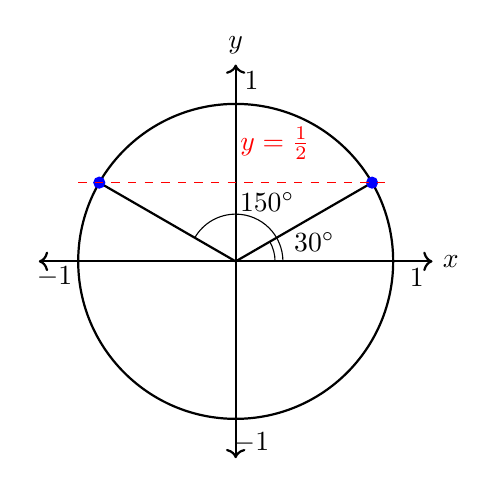
\begin{tikzpicture}
        % Draw unit circle
        \draw[thick] (0,0) circle (2);

        % Draw axes
        \draw[<->, thick] (-2.5,0) -- (2.5,0) node[right] {$x$};
        \draw[<->, thick] (0,-2.5) -- (0,2.5) node[above] {$y$};

        % Mark unit circle points
        \node at (2.3,-0.2) {$1$};
        \node at (-2.3,-0.2) {$-1$};
        \node at (0.2,2.3) {$1$};
        \node at (0.2,-2.3) {$-1$};

        % Draw radius lines for 30 degrees
        \draw[thick] (0,0) -- ({2*cos(30)},{2*sin(30)});
        \draw[thick] (0,0) -- ({2*cos(150)},{2*sin(150)});

        % Mark points on the circle
        \filldraw[blue] ({2*cos(30)},{2*sin(30)}) circle (0.07);
        \filldraw[blue] ({2*cos(150)},{2*sin(150)}) circle (0.07);

        % Draw horizontal line for y = 1
        \draw[dashed, red] (-2,1) -- (2,1);
        \node[red] at (0.5,1.5) {$y = \frac{1}{2}$};

        % Mark angles
        \draw (0.5,0) arc (0:30:0.5);
        \node at (1,0.25) {$30^\circ$};

        \draw (0.6,0) arc (0:150:0.6);
        \node at (0.4,0.75) {$150^\circ$};
    \end{tikzpicture}
\end{center}

Stejně tak můžeme určit úhel i pro goniometrickou funkci kosinus.
Například chceme-li najít úhel, pro který platí $\cos x = -\frac{1}{2}$.
Z tabulky vidíme, že $\cos 120^\circ = -\frac{1}{2}$,
takže jedním z řešení je $x = 120^\circ$. Když si však opět nakreslíme jednotkovou kružnici,
vidíme, že existuje ještě jedno řešení v třetím kvadrantu, a to $x = 240^\circ$,
protože $\cos 240^\circ = -\frac{1}{2}$ také platí. Obecně tedy platí, že pro $\cos x = -\frac{1}{2}$
jsou řešení ve tvaru:
\[x_1 = 120^\circ, \quad \text{a} \quad  x_2 = 240^\circ\]

\begin{center}
    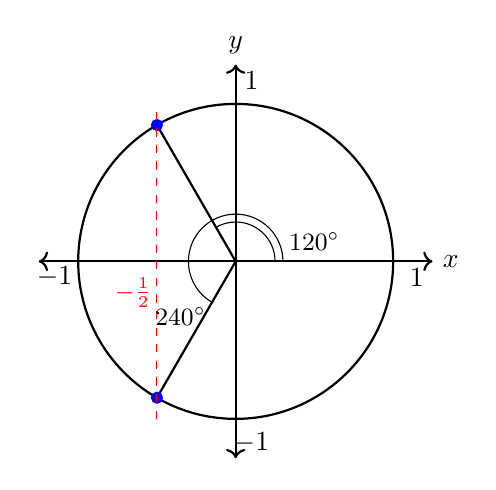
\begin{tikzpicture}
        % Draw unit circle
        \draw[thick] (0,0) circle (2);

        % Draw axes
        \draw[<->, thick] (-2.5,0) -- (2.5,0) node[right] {$x$};
        \draw[<->, thick] (0,-2.5) -- (0,2.5) node[above] {$y$};

        % Mark unit circle points
        \node at (2.3,-0.2) {$1$};
        \node at (-2.3,-0.2) {$-1$};
        \node at (0.2,2.3) {$1$};
        \node at (0.2,-2.3) {$-1$};

        % Draw radius lines for 120 degrees
        \draw[thick] (0,0) -- ({2*cos(120)},{2*sin(120)});
        \draw[thick] (0,0) -- ({2*cos(240)},{2*sin(240)});

        % Mark points on the circle
        \filldraw[blue] ({2*cos(120)},{2*sin(120)}) circle (0.07);
        \filldraw[blue] ({2*cos(240)},{2*sin(240)}) circle (0.07);

        % Draw vertical line for x = -1/2
        \draw[dashed, red] (-1, -2) -- (-1, 2);
        \node[red] at (-1.3,-0.4) {\small $-\frac{1}{2}$};

        % Mark angles
        \draw (0.5,0) arc (0:120:0.5);
        \node at (1,0.25) {\small $120^\circ$};

        \draw (0.6,0) arc (0:240:0.6);
        \node at (-0.7,-0.7) {\small $240^\circ$};
    \end{tikzpicture}
\end{center}

A jsou tyto dvě hodnoty jediné možné?
Ne, protože můžeme najít nekonečně mnoho dalších řešení přidáním celých násobků $360^\circ$.
Což jde dobře vidět na grafech goniometrických funkcí, které jsou periodické, právě po $360^\circ$ pro sinus a kosinus.
Nebo po $180^\circ$ pro tangens a cotangens.
To znamená, že pokud $x$ je řešením rovnice pro sinus a kosinus, pak i $x + 360^\circ k$ je také řešením, kde $k$ je libovolné celé číslo.
A obdobně pro tangens a cotangens, pokud $x$ je řešením, pak i $x + 180^\circ k$ je také řešením, kde $k$ je libovolné celé číslo.
Což jde vidět i z následujícího grafu funkce $\sin x$.

\begin{center}
    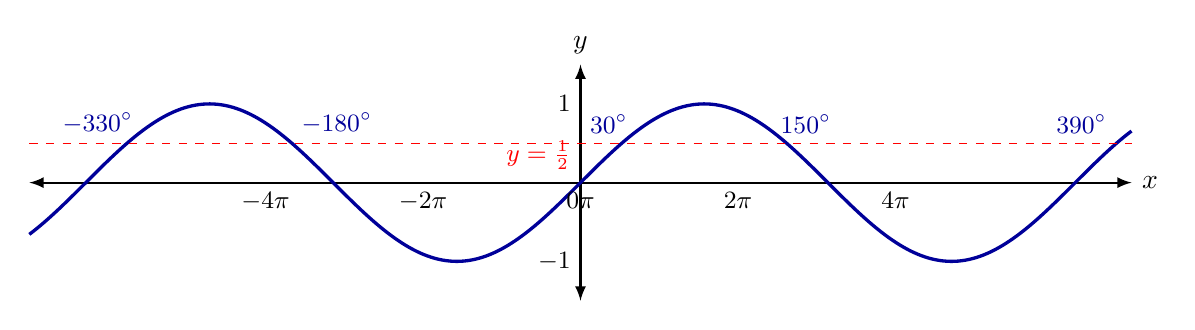
\begin{tikzpicture}[scale=1, >=latex]
        
        % ==== AXES ====
        \draw[<->, thick] (-7,0) -- (7,0) node[right] {$x$};
        \draw[<->, thick] (0,-1.5) -- (0,1.5) node[above] {$y$};
        
        % ==== SIN CURVE ====
        \draw[very thick, blue!60!black, samples=300, domain=-7:7]
            plot(\x,{sin(\x r)});
        
         % ==== HORIZONTAL LINE y=1/2 ====
        \draw[dashed, red] (-7,0.5) -- (7,0.5);

        % ==== NODES ON AXIS ====
        \foreach \k in {-4,-2,0,2,4}{
            \node[below] at (\k,0) {\small $\k\pi$};
        }

        % ==== NODES ON CURVE ====
        \node[above left, blue!60!black] at (pi/6+0.2, 0.5) {\small $30^\circ$};
        \node[above right, blue!60!black] at (5*pi/6-0.2, 0.5) {\small $150^\circ$};
        \node[above left, blue!60!black] at (pi/6 +2*pi, 0.5) {\small $390^\circ$};
        \node[above left, blue!60!black] at (pi/6 -2*pi+0.2, 0.5) {\small $-330^\circ$};
        \node[above right, blue!60!black] at (5*pi/6 -2*pi, 0.5) {\small $-180^\circ$};

        % ==== NODE ON Y-AXIS ====
        \node[below left, red] at (0,0.66) {\small $y = \frac{1}{2}$};
        \node[left] at (0,1) {\small $1$};
        \node[left] at (0,-1) {\small $-1$};

    \end{tikzpicture}

\end{center}

z grafu této funkce můžeme vidět, že hodnota $\sin x = \frac{1}{2}$ nastává v nekonečně mnoha bodech,
které odpovídají úhlům $30^\circ + 360^\circ k$ a $150^\circ + 360^\circ k$, kde $k$ je libovolné celé číslo. 
Což můžeme zapsat jako obecné řešení rovnice $\sin x = \frac{1}{2}$ pomocí množiny bodů:
\[
x = \{30^\circ + 360^\circ k,\, 150^\circ + 360^\circ k ; k \in \mathbb{Z} \}.
\]
nebo jako pomocí radiánů:
\[
x = \left\{\frac{\pi}{6} + 2\pi k,\, \frac{5\pi}{6} + 2\pi k ; k \in \mathbb{Z} \right\}.
\]

S tímto zápisem se setkáme i v další kapitole o \important{goniometrických rovnicích a nerovnicích}.


\subsection{Stupňová, oblouková a úseková míra úhlu}
Jak jste si možná všimli, v této kapitole jsme používali jak \important{stupňovou}, tak \important{radiánovou} míru úhlu.
Radiánová míra je v matematice preferována, protože vede k jednodušším a elegantnějším vzorcům
a usnadňuje práci s goniometrickými funkcemi v pokročilejších oblastech matematiky, jako je analýza
a diferenciální rovnice. Stupňová míra je však často používána v praktických aplikacích a v některých oborech,
jako je navigace a geografie, kde je intuitivnější pro měření úhlů.

\subsubsection*{Stupňová míra}
\important{Stupňová míra úhlu} je založena na rozdělení celého kruhu na $360$ stejných částí, zvaných stupně.
Tento systém má historické kořeny sahající až do starověkých civilizací, které používaly
360denní kalendář a astronomická pozorování. Jeden stupeň je tedy definován jako $\frac{1}{360}$ celého kruhu.
Pro jemnější měření úhlů se používají také \textbf{minuty} a \textbf{sekundy}, kde jeden stupeň se dělí na
$60$ minut a jedna minuta na $60$ sekund:
\[1^\circ = 60' \quad\text{a}\quad 1' = 60''.\]


\subsubsection*{Oblouková míra}
\important{Oblouková míra úhlu} je definována jako délka oblouku na jednotkové kružnici, který tento úhel svírá.
Jeden radián je úhel, který svírá oblouk délky rovné poloměru jednotkové kružnice, tedy délce $1$.
Celý kruh má obvod $2\pi$, což znamená, že celý kruh odpovídá úhlu $2\pi$ radiánů.

\begin{center}
    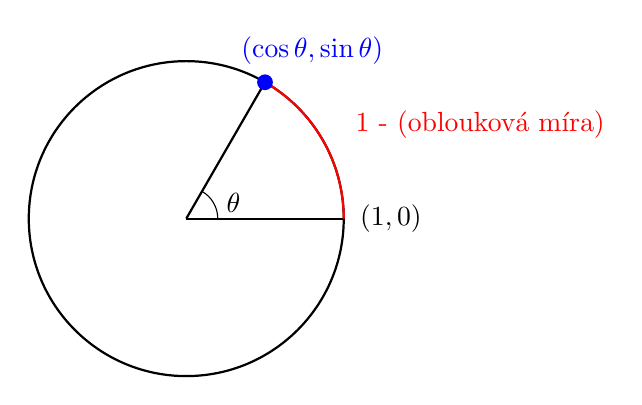
\begin{tikzpicture}[scale=2,>=latex]

        % Draw unit circle
        \draw[thick] (0,0) circle (1);

        % Draw radius lines
        \draw[thick] (0,0) -- (1,0); % 0 radians
        \draw[thick] (0,0) -- ({cos(60)},{sin(60)}); % 60 degrees

        % Draw arc for 60 degrees
        \draw[thick, red] (1,0) arc (0:60:1);
        \node[red] at ({cos(30)+1},{sin(30)+0.1}) {1 - (oblouková míra)};

        % Mark angle
        \draw (0.2,0) arc (0:60:0.2);
        \node at (0.3,0.1) {$\theta$};

        % Labels
        \node at (1.3,0) {$(1,0)$};
        \fill[blue] ({cos(60)},{sin(60)}) circle (0.05);
        \node[blue] at ({cos(60)+0.3},{sin(60)+0.2}) {$(\cos\theta,\sin\theta)$};

    \end{tikzpicture}
\end{center}

Jak zjistit obloukovou míru úhlu v radiánech, pokud je úhel dán ve stupních?
Použijeme převodní vztah mezi stupni a radiány, který vychází z faktu, že celý kruh má $360^\circ$ nebo $2\pi$ radiánů a trojčlenky:

\begin{definitionbox}
\[\text{oblouková míra (v radiánech)} = \frac{\pi}{180^\circ} \cdot \text{úhel (ve stupních)}.\]
\end{definitionbox}

\begin{examplebox}
Například úhel, který má $60^\circ$ má obloukovou míru:
\[\frac{\pi}{180^\circ} \times 60^\circ = \frac{\pi}{3} \text{ radiánů}.\]
\end{examplebox}


\subsubsection*{Úseková míra}
\important{Úseková míra úhlu} je méně běžný způsob měření úhlů, který se používá především v některých technických a inženýrských aplikacích. 
V tomto systému je úhel měřen jako délka přímé čáry (úseku) spojující dva body na kružnici, které jsou spojeny daným úhlem.
Úseková míra je tedy vzdálenost mezi dvěma body na kružnici, které jsou spojeny úhlem, měřená podél přímé čáry, nikoli podél oblouku kružnice.
Tento způsob měření úhlů není tak běžný jako stupňová nebo oblouková míra, ale může být užitečný v určitých kontextech, například při analýze geometrických tvarů nebo konstrukci mechanismů.

\begin{examplebox}
Například pokud máme úhel $60^\circ$ na jednotkové kružnici, úseková míra tohoto úhlu je délka přímé čáry spojující bod $(1,0)$ a bod odpovídající $60^\circ$, což je přibližně $1.732$.
\end{examplebox}

Nicméně s touto mírou se v běžné matematice a fyzice příliš nesetkáme, a proto se jí nebudeme více věnovat.



\subsection*{Orientovaný úhel}

V goniometrii je důležité rozlišovat mezi \textbf{orientovanými} a \textbf{neorientovanými} úhly.
\important{Orientovaný úhel} má přiřazen směr otáčení, který určuje, zda je úhel kladný nebo záporný.
Kladný orientovaný úhel se měří proti směru hodinových ručiček (obvykle se jedná o pohyb z kladné části osy $x$ směrem k ose $y$),
zatímco záporný orientovaný úhel se měří ve směru hodinových ručiček.

Úhly díky tomu, že jsou orientované, mohou nabývat i záporných hodnot a hodnot větších než $360^\circ$ (nebo $2\pi$ radiánů).
To umožňuje popsat více než jednu otáčku kolem kružnice a také vyjádřit směr otáčení.

\begin{examplebox}
    Například úhel $450^\circ$ je orientovaný úhel, který představuje jednu celou otáčku ($360^\circ$) plus další $90^\circ$ proti směru hodinových ručiček.
    Tento úhel je ekvivalentní orientovanému úhlu $90^\circ$.
    Můžeme tedy napsat, že:
    \[
    450^\circ = 90^\circ + 360^\circ = 90^\circ = \frac{\pi}{2} \text{ radiánů},
    \]
    nebo taky:
    \[
    -760^\circ = -400^\circ + 360^\circ = -40^\circ + 360^\circ + 360^\circ = -40^\circ = -\frac{2\pi}{9} \text{ radiánů}.
    \]
\end{examplebox}

Jak ale zjistit velikost úhlů, které jsou příliš veliké? 
Pro zjištění velikosti orientovaného úhlu, který je větší než $360^\circ$, využijeme faktu, že se perioda opakuje po $360^\circ$.
A tedy stačí když požadovaný úhel vydělíme $360^\circ$ a zbytek nám dá velikost úhlu v intervalu $\langle 0^\circ, 360^\circ)$.

\begin{examplebox}
    Chceme zjistit velikost úhlů $15327^\circ$.
    Pro úhel $15327^\circ$ tedy provedeme následující výpočet:
    \[
    \frac{15327}{360} = 42.575
    \]
    Celé číslo zde reprezentuje počet otáček, které úhel obsahuje, a desetinná část nám říká, jak velký je zbytek úhlu po odečtení celých otáček.
    Násobíme tedy desetinnou část $0.575$ zpět $360^\circ$:
    \[0.575 \times 360^\circ = 207^\circ.\]
    Tedy velikost orientovaného úhlu $15327^\circ$ je $207^\circ$.
\end{examplebox}

Nyní když spojíme poznatky o orientovaných úhlech s jednotkovou kružnicí, můžeme snadno určit hodnoty goniometrických funkcí
i pro úhly mimo interval $\langle 0, 2\pi)$ (nebo $\langle 0^\circ, 360^\circ)$). Stačí najít odpovídající úhel v tomto intervalu a použít jeho hodnoty.    

Zároveň díky faktu, že jednotková kružnice má poloměr jedna $r=1$ můžeme jednoduše určit hodnoty goniometrických funkcí pomocí právě jednotkové kružnice.
Stejně jako jsme je odvozovali pomocí pravoúhlého trojúhelníku, můžeme je nyní odvodit přímo z jednotkové kružnice.
A sice tak, že si představíme pravoúhlý trojúhelník, který vznikne spojením středu kružnice,
počátku osy $x$ a bodu na kružnici odpovídajícímu úhlu $\varphi$.

\begin{center}
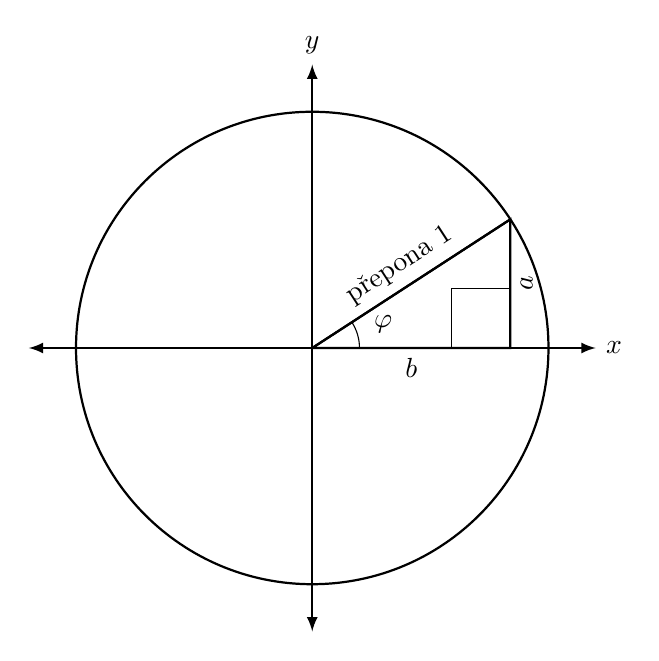
\begin{tikzpicture}[scale=3,>=latex]
    % Draw unit circle
    \draw[thick] (0,0) circle (1);

    % Draw radius line for angle φ
    \coordinate (P) at ({cos(33)},{sin(33)});
    \draw[thick] (0,0) -- node[midway,sloped,above] { } (P);

    % Draw x and y axes
    \draw[<->, thick] (-1.2,0) -- (1.2,0) node[right] {$x$};
    \draw[<->, thick] (0,-1.2) -- (0,1.2) node[above] {$y$};

    % Draw right triangle
    \coordinate (A) at (0,0);
    \coordinate (B) at ({cos(33)},0);
    \coordinate (C) at ({cos(33)},{sin(33)});
    \draw[thick] (A) -- node[midway,below] {$b$} (B)
    -- node[midway,sloped,below] {$a$} (C)
    -- node[midway,sloped,above] {přepona $1$} (A);
    \tkzMarkRightAngle (A,B,C);
    % Angle label
    \draw (0.2,0) arc (0:33:0.2);
    \node at (0.3,0.1) {$\varphi$};
\end{tikzpicture}
\end{center}

Z tohoto trojúhelníku nyní můžeme odvodit hodnoty goniometrických funkcí:
\begin{itemize}
    \item $\sin\varphi = \dfrac{\text{protilehlá odvěsna}}{\text{přepona}} = \dfrac{a}{1} = a = y$,
    \item $\cos\varphi = \dfrac{\text{přilehlá odvěsna}}{\text{přepona}} = \dfrac{b}{1} = b = x$,
    \item $\tan\varphi = \dfrac{\sin\varphi}{\cos\varphi} = \dfrac{a}{b} = \dfrac{y}{x}$, \qquad $\cot\varphi = \dfrac{\cos\varphi}{\sin\varphi} = \dfrac{b}{a} = \dfrac{x}{y}$.
\end{itemize}


\section{Vlastnsoti goniometrických funkcí}
Jak jsme si nazačátku této kapitoly ukázali, goniometrické funkce mají řadu zajímavých vlastností.
Nyní si je však rozebere podrobněji.

\subsection{Periodičnost}
Goniometrické funkce jsou periodické, což znamená, že jejich hodnoty se opakují v pravidelných intervalech.
Pro funkce sinus a kosinus je perioda $2\pi$, což znamená, že pro každé reálné číslo $x$ platí:
\[\sin(x + 2\pi) = \sin x,\]
\[\cos(x + 2\pi) = \cos x.\]

A zároveň tedy víme, že hodnoty funkcí sinus a kosinus nejsou jen omezeny na interval $\langle 0, 2\pi)$,
ale můžeme je určit pro libovolné reálné číslo $x$. Proto z toho plyne, že \important{definiční obor} funkcí sinus a kosinus je množina všech reálných čísel $\mathbb{R}$.

\begin{center}
    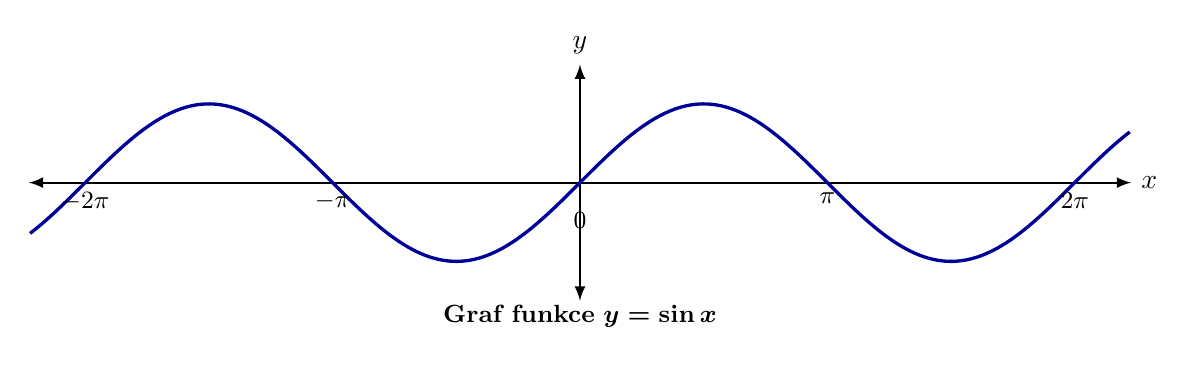
\begin{tikzpicture}[scale=1, >=latex]
        % ==== AXES ====
        \draw[<->, thick] (-7,0) -- (7,0) node[right] {$x$};
        \draw[<->, thick] (0,-1.5) -- (0,1.5) node[above] {$y$};
        % ==== SINUS CURVE ====
        \draw[very thick, blue!60!black, samples=300, domain=-2*pi-0.7:2*pi+0.7]
            plot(\x,{sin(\x r)});
        \node[below] at (0,-0.25) {\small $0$};
        \node[below] at ({-2*pi},0) {\small $-2\pi$};
        \node[below] at ({-pi},0) {\small $-\pi$};
        \node[below] at ({pi},0) {\small $\pi$};
        \node[below] at ({2*pi},0) {\small $2\pi$};
       
        % ==== Title ====
        \node at (0,-1.7) {\small \textbf{Graf funkce} $\boldsymbol{y = \sin x}$};
     \end{tikzpicture}
\end{center}

\begin{center}
    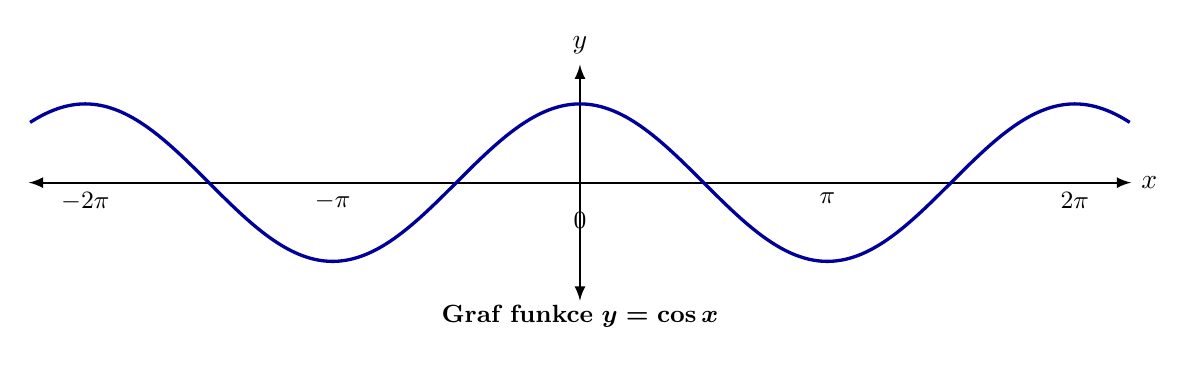
\begin{tikzpicture}[scale=1, >=latex]
        % ==== AXES ====
        \draw[<->, thick] (-7,0) -- (7,0) node[right] {$x$};
        \draw[<->, thick] (0,-1.5) -- (0,1.5) node[above] {$y$};
        % ==== COSINUS CURVE ====
        \draw[very thick, blue!60!black, samples=300, domain=-2*pi-0.7:2*pi+0.7]
            plot(\x,{cos(\x r)});
        \node[below] at (0,-0.25) {\small $0$};
        \node[below] at ({-2*pi},0) {\small $-2\pi$};
        \node[below] at ({-pi},0) {\small $-\pi$};
        \node[below] at ({pi},0) {\small $\pi$};
        \node[below] at ({2*pi},0) {\small $2\pi$};
       
        % ==== Title ====
        \node at (0,-1.7) {\small \textbf{Graf funkce} $\boldsymbol{y = \cos x}$};
     \end{tikzpicture}
\end{center}


Tangens a kotangens mají periodu $\pi$, což znamená, že pro každé reálné číslo $x$ platí:
\[\tan(x + \pi) = \tan x,\]
\[\cot(x + \pi) = \cot x.\]
Opět tedy platí, že hodnoty funkcí tangens a kotangens můžeme určit pro libovolné reálné číslo $x$.
Z toho plyne, že \important{definiční obor} funkcí tangens a kotangens je také množina všech reálných čísel $\mathbb{R}$,
s výjimkou těch hodnot, pro které jsou tyto funkce nedefinované (kde je kosinus nebo sinus rovný nule).
Tedy pro tangens jsou to hodnoty $x = \frac{\pi}{2} + k\pi$, kde $k$ je celé číslo, a pro kotangens jsou to hodnoty $x = k\pi$.
Definiční obory tedy můžeme zapsat jako:
\[D(f)_{\tan} = \mathbb{R} \setminus \left\{ \frac{\pi}{2} + k\pi \mid k \in \mathbb{Z} \right\},\]
\[D(f)_{\cot} = \mathbb{R} \setminus \left\{ k\pi \mid k \in \mathbb{Z} \right\}.\]

\subsection{Sudost a lichost goniometrických funkcí}
Goniometrické funkce mají také vlastnosti sudosti a lichosti:
\begin{itemize}
    \item Funkce \textbf{sinus}, \textbf{tangens} a \textbf{kotangens} jsou \important{liché funkce}, což znamená, že pro každé reálné číslo $x$ platí:
    \[\sin(-x) = -\sin x,\]
    \[\tan(-x) = -\tan x,\]
    \[\cot(-x) = -\cot x.\]
    \item Funkce \textbf{kosinus} je \important{sudá funkce}, což znamená, že pro každé reálné číslo $x$ platí:
    \[\cos(-x) = \cos x.\]
\end{itemize}

Tato vlastnost sudosti a lichosti je užitečná při analýze grafů goniometrických funkcí a při řešení goniometrických rovnic (se kterými se setákme v další kapitole).

\subsection{Posuny goniometrických funkcí}
Jak si lze všimnou z grafu funkcí, tak sinus jako kosinus mají charakteristické posuny.
Funkce kosinus je posunuta o $\frac{\pi}{2}$ doleva vůči funkci sinus.
To znamená, že můžeme vyjádřit kosinus pomocí sinu s posunem:
\[\cos x = \sin\left(x + \frac{\pi}{2}\right).\]
Podobně můžeme vyjádřit sinus pomocí kosinu s posunem:
\[\sin x = \cos\left(x - \frac{\pi}{2}\right).\]

Stejně tak můžeme vyjádřit tangens pomocí kotangens s posunem:
\[\tan x = \cot\left(x - \frac{\pi}{2}\right),\]
a kotangens pomocí tangens s posunem:
\[\cot x = \tan\left(x + \frac{\pi}{2}\right).\]


\newpage
\section{Grafy goniometrických funkcí}

Prvně si znovu připomeneme grafy jednotlivých goniometrických funkcí.

\smallskip
Funkce \textbf{sinus}:
\begin{center}
    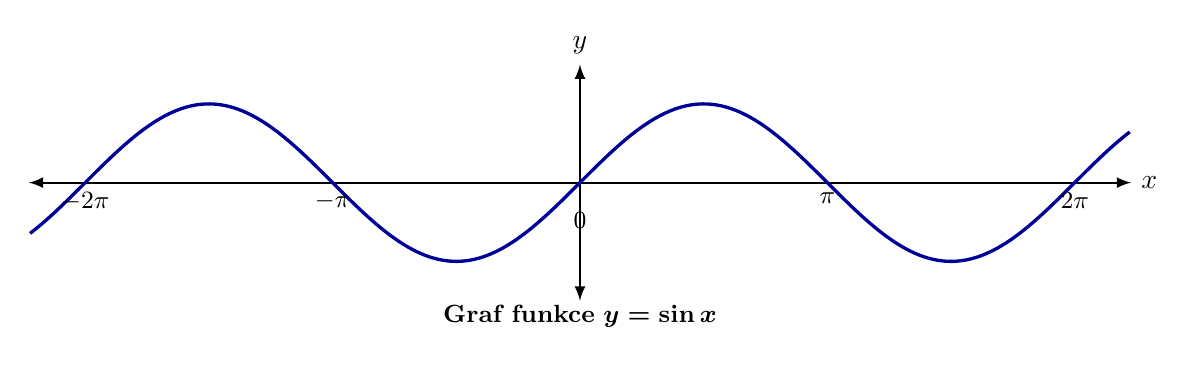
\begin{tikzpicture}[scale=1, >=latex]
        % ==== AXES ====
        \draw[<->, thick] (-7,0) -- (7,0) node[right] {$x$};
        \draw[<->, thick] (0,-1.5) -- (0,1.5) node[above] {$y$};
        % ==== SINUS CURVE ====
        \draw[very thick, blue!60!black, samples=300, domain=-2*pi-0.7:2*pi+0.7]
            plot(\x,{sin(\x r)});
        \node[below] at (0,-0.25) {\small $0$};
        \node[below] at ({-2*pi},0) {\small $-2\pi$};
        \node[below] at ({-pi},0) {\small $-\pi$};
        \node[below] at ({pi},0) {\small $\pi$};
        \node[below] at ({2*pi},0) {\small $2\pi$};
       
        % ==== Title ====
        \node at (0,-1.7) {\small \textbf{Graf funkce} $\boldsymbol{y = \sin x}$};
     \end{tikzpicture}
\end{center}


Tento graf ukazuje goniometrickou funkci sinus. Nicméně ne vždy je potřeba základní graf funkce sinus.
Často se setkáváme s různými úpravami této funkce, které zahrnují změny amplitudy, periodičnosti a posunu.
Obecná rovnice pro takovou upravenou funkci sinus je následující:
\[y = a \sin(b(x - c)) + d,\]
kde:
\begin{itemize}
    \item $a$ je amplituda (vertikální rozměr vlny),
    \item $b$ ovlivňuje periodu (horizontální rozměr vlny),
    \item $c$ je horizontální posun (fáze),
    \item $d$ je vertikální posun.
\end{itemize}

\begin{examplebox}
Uvažujme funkci:
\[y = 2 \sin\left(3x - \frac{\pi}{4}\right) + 1.\]
Graf této funkce budeme vytvářet postupným přidáváním jednotlivých úprav k základnímu grafu funkce sinus.
\begin{enumerate}[label=\arabic*.]
    \item Začneme s grafem základní funkce $y = \sin x$.
    \item Následně aplikujeme změnu amplitudy na $a = 2$, což znamená, že graf bude roztažen vertikálně o faktor $2$.
    \item Dále upravíme periodu pomocí $b = 3$. Perioda se vypočítá jako $\frac{2\pi}{b} = \frac{2\pi}{3}$, což znamená, že graf bude stlačen horizontálně.
    \item Poté provedeme horizontální posun o $c = \frac{\pi}{4}$ doprava.
    \item Nakonec přidáme vertikální posun o $d = 1$, což znamená, že celý graf se posune o $1$ jednotku nahoru.
\end{enumerate}

\newpage
\textbf{1. Základní graf:}
\begin{center}
    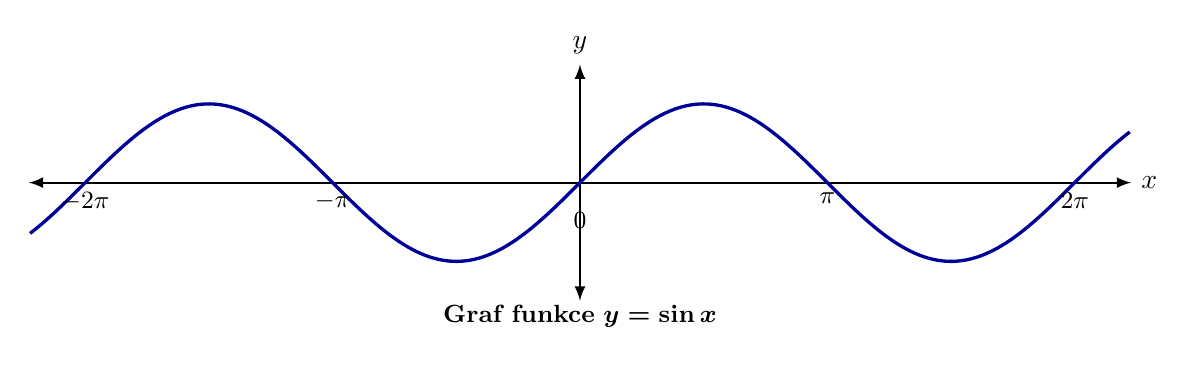
\begin{tikzpicture}[scale=1, >=latex]
        % ==== AXES ====
        \draw[<->, thick] (-7,0) -- (7,0) node[right] {$x$};
        \draw[<->, thick] (0,-1.5) -- (0,1.5) node[above] {$y$};
        % ==== SINUS CURVE ====
        \draw[very thick, blue!60!black, samples=300, domain=-2*pi-0.7:2*pi+0.7]
            plot(\x,{sin(\x r)});
        \node[below] at (0,-0.25) {\small $0$};
        \node[below] at ({-2*pi},0) {\small $-2\pi$};
        \node[below] at ({-pi},0) {\small $-\pi$};
        \node[below] at ({pi},0) {\small $\pi$};
        \node[below] at ({2*pi},0) {\small $2\pi$};
       
        % ==== Title ====
        \node at (0,-1.7) {\small \textbf{Graf funkce} $\boldsymbol{y = \sin x}$};
     \end{tikzpicture}
\end{center}

\bigskip
\textbf{2. Po změně amplitudy na $a = 2$:}
\begin{center}
    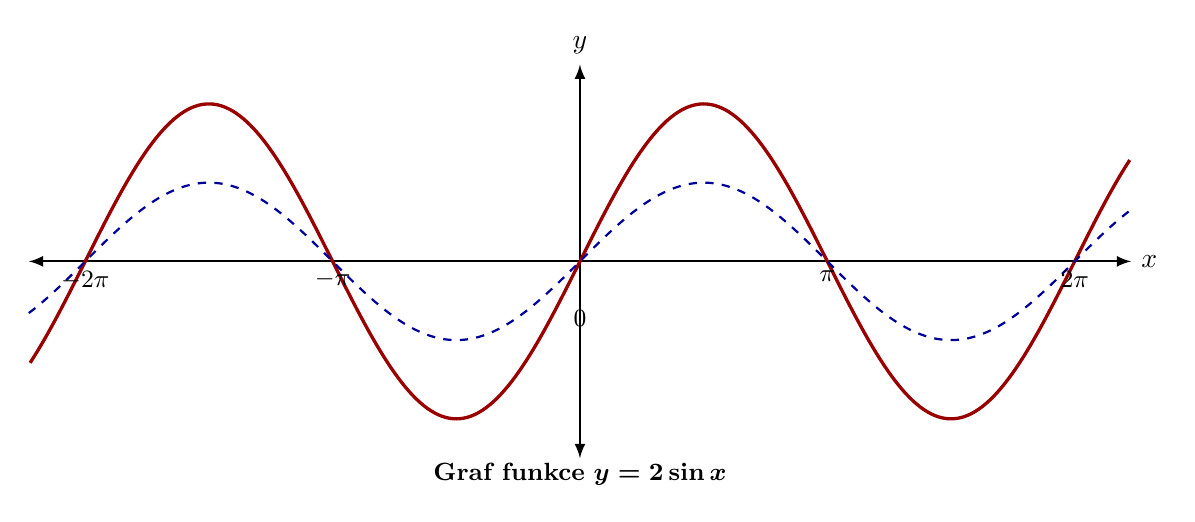
\begin{tikzpicture}[scale=1, >=latex]
        % ==== AXES ====
        \draw[<->, thick] (-7,0) -- (7,0) node[right] {$x$};
        \draw[<->, thick] (0,-2.5) -- (0,2.5) node[above] {$y$};
        % ==== SINUS CURVE WITH AMPLITUDE 2 ====
        \draw[very thick, red!60!black, samples=300, domain=-2*pi-0.7:2*pi+0.7]
            plot(\x,{2*sin(\x r)});
        \draw[thick, blue!60!black, dashed, samples=300, domain=-7:7]
            plot(\x,{sin(\x r)});
        \node[below] at (0,-0.5) {\small $0$};
        \node[below] at ({-2*pi},0) {\small $-2\pi$};
        \node[below] at ({-pi},0) {\small $-\pi$};
        \node[below] at ({pi},0) {\small $\pi$};
        \node[below] at ({2*pi},0) {\small $2\pi$};
       
        % ==== Title ====
        \node at (0,-2.7) {\small \textbf{Graf funkce} $\boldsymbol{y = 2\sin x}$};
     \end{tikzpicture}
\end{center}

\bigskip
\textbf{3. Po úpravě periody na $b = 3$:}
\begin{center}
    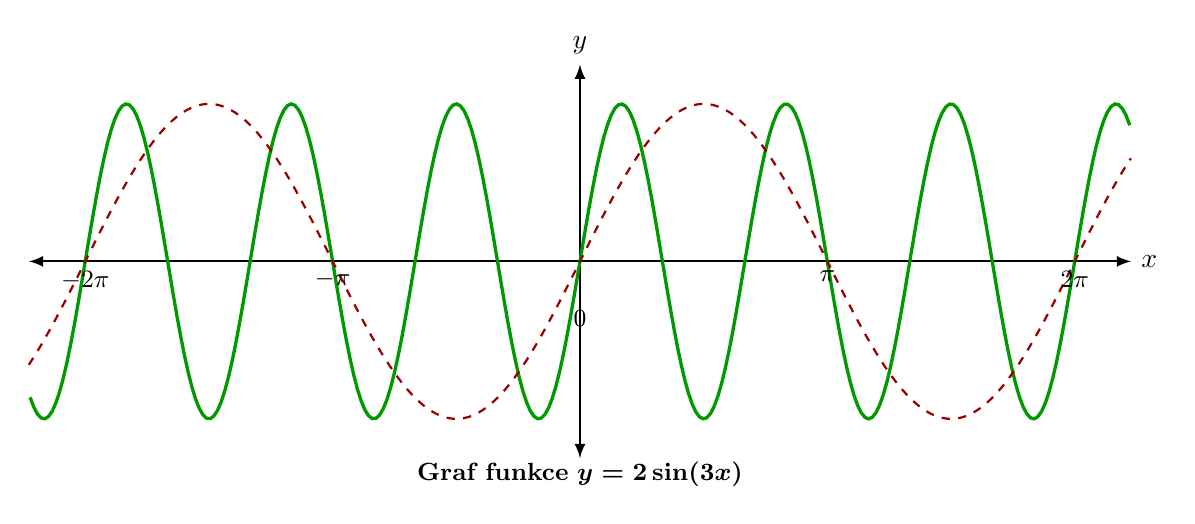
\begin{tikzpicture}[scale=1, >=latex]
        % ==== AXES ====
        \draw[<->, thick] (-7,0) -- (7,0) node[right] {$x$};
        \draw[<->, thick] (0,-2.5) -- (0,2.5) node[above] {$y$};
        % ==== SINUS CURVE WITH AMPLITUDE 2 AND PERIOD 2π/3 ====
        \draw[very thick, green!60!black, samples=300, domain=-2*pi-0.7:2*pi+0.7]
            plot(\x,{2*sin(3*\x r)});
        \draw[thick, red!60!black, dashed, samples=300, domain=-7:7]
            plot(\x,{2*sin(\x r)});
        \node[below] at (0,-0.5) {\small $0$};
        \node[below] at ({-2*pi},0) {\small $-2\pi$};
        \node[below] at ({-pi},0) {\small $-\pi$};
        \node[below] at ({pi},0) {\small $\pi$};
        \node[below] at ({2*pi},0) {\small $2\pi$};
       
        % ==== Title ====
        \node at (0,-2.7) {\small \textbf{Graf funkce} $\boldsymbol{y = 2\sin(3x)}$};
     \end{tikzpicture}
\end{center}
Po vynásobení $x$ koeficientem $3$ se perioda zmenšila na $\frac{2\pi}{3}$. 
Neboli v původním grafu, kde jedna perioda trvala $2\pi$, nyní trvá pouze $\frac{2\pi}{3}$.

\newpage
\textbf{4. Po horizontálním posunu o $c = \frac{\pi}{4}$ doprava:}
\begin{center}
    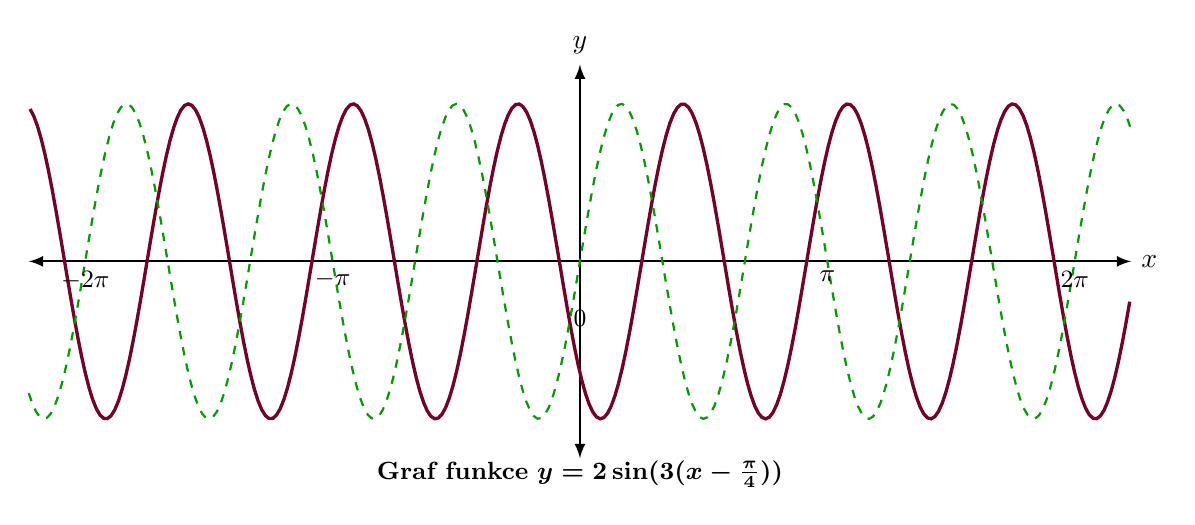
\begin{tikzpicture}[scale=1, >=latex]
        % ==== AXES ====
        \draw[<->, thick] (-7,0) -- (7,0) node[right] {$x$};
        \draw[<->, thick] (0,-2.5) -- (0,2.5) node[above] {$y$};
        % ==== SINUS CURVE WITH AMPLITUDE 2, PERIOD 2π/3 AND HORIZONTAL SHIFT π/4 ====
        \draw[very thick, purple!60!black, samples=300, domain=-2*pi-0.7:2*pi+0.7]
            plot(\x,{2*sin(3*(\x - pi/4) r)});
        \draw[thick, green!60!black, dashed, samples=300, domain=-7:7]
            plot(\x,{2*sin(3*\x r)});
        \node[below] at (0,-0.5) {\small $0$};
        \node[below] at ({-2*pi},0) {\small $-2\pi$};
        \node[below] at ({-pi},0) {\small $-\pi$};
        \node[below] at ({pi},0) {\small $\pi$};
        \node[below] at ({2*pi},0) {\small $2\pi$};
       
        % ==== Title ====
        \node at (0,-2.7) {\small \textbf{Graf funkce} $\boldsymbol{y = 2\sin(3(x - \frac{\pi}{4}))}$};
     \end{tikzpicture}
\end{center}
Po posunu o $\frac{\pi}{4}$ doprava se celý graf posunul o tuto hodnotu na ose $x$.

\bigskip
\textbf{5. Po vertikálním posunu o $d = 1$ nahoru:}
\begin{center}
    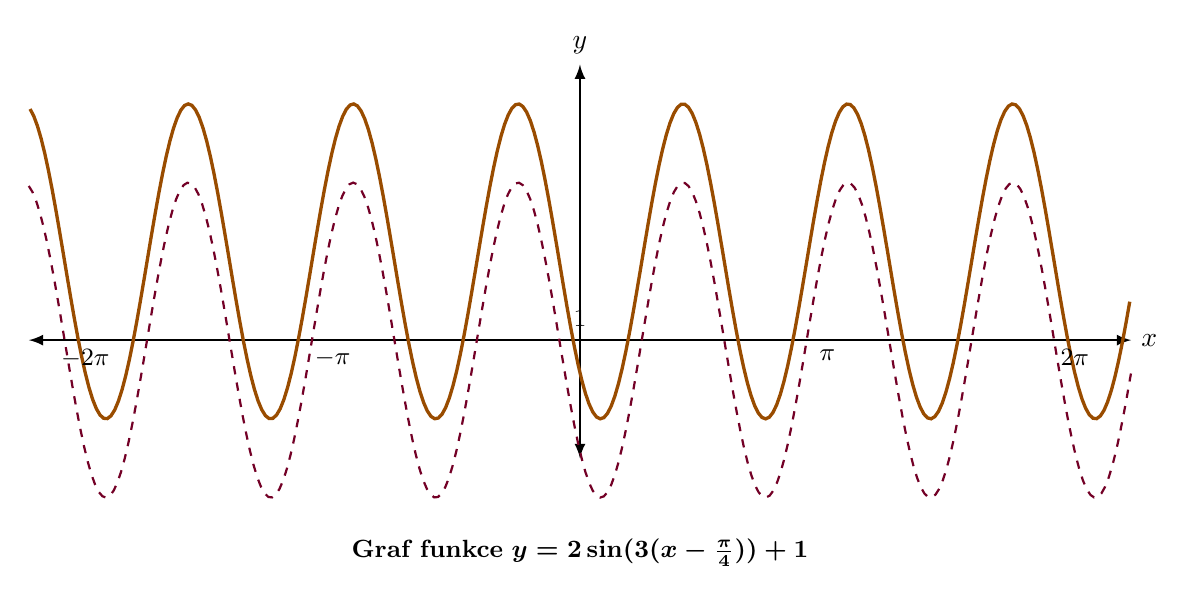
\begin{tikzpicture}[scale=1, >=latex]
        % ==== AXES ====
        \draw[<->, thick] (-7,0) -- (7,0) node[right] {$x$};
        \draw[<->, thick] (0,-1.5) -- (0,3.5) node[above] {$y$};
        % ==== SINUS CURVE WITH AMPLITUDE 2, PERIOD 2π/3, HORIZONTAL SHIFT π/4 AND VERTICAL SHIFT 1 ====
        \draw[very thick, orange!60!black, samples=300, domain=-2*pi-0.7:2*pi+0.7]
            plot(\x,{2*sin(3*(\x - pi/4) r) + 1});
        \draw[thick, purple!60!black, dashed, samples=300, domain=-7:7]
            plot(\x,{2*sin(3*(\x - pi/4) r)});
        \node[below] at (0,0.5) {\small $1$};
        \node[below] at ({-2*pi},0) {\small $-2\pi$};
        \node[below] at ({-pi},0) {\small $-\pi$};
        \node[below] at ({pi},0) {\small $\pi$};
        \node[below] at ({2*pi},0) {\small $2\pi$};
       
        % ==== Title ====
        \node at (0,-2.7) {\small \textbf{Graf funkce} $\boldsymbol{y = 2\sin(3(x - \frac{\pi}{4})) + 1}$};
     \end{tikzpicture}
\end{center}
Po posunu o $1$ nahoru se celý graf posunul o tuto hodnotu na ose $y$.
Tímto jsme dokončili konstrukci grafu funkce
\end{examplebox}

Tímto způsobem můžeme vytvářet grafy různých goniometrických funkcí s různými úpravami.
Můžeme se však setka také s funkcemi, které jsou umocněny, nebo naopak odmocněny.
Například funkce jako $y = \sin^2 x$ nebo $y = \sqrt{\cos x}$.
A konstrukce těchto grafů si nyní ukážeme na příkladech.

\begin{examplebox}
    Mějme funkci:
    \[y = \sin^2 x.\]
    Tento graf můžeme vytvořit tak, že nejprve nakreslíme základní graf funkce $y = \sin x$,
    a poté pro každé $x$ na ose $x$ umocníme hodnotu $y$ na druhou.
    To znamená, že pokud je hodnota $y$ kladná, zůstane stejná, ale pokud je hodnota $y$ záporná, stane se kladnou.

    \textbf{1. Základní graf:}
    \begin{center}
        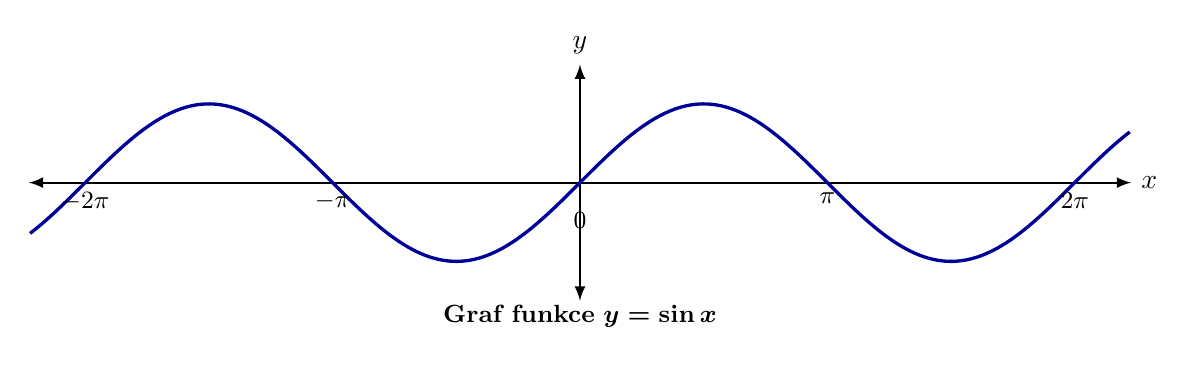
\begin{tikzpicture}[scale=1, >=latex]
            % ==== AXES ====
            \draw[<->, thick] (-7,0) -- (7,0) node[right] {$x$};
            \draw[<->, thick] (0,-1.5) -- (0,1.5) node[above] {$y$};
            % ==== SINUS CURVE ====
            \draw[very thick, blue!60!black, samples=300, domain=-2*pi-0.7:2*pi+0.7]
                plot(\x,{sin(\x r)});
            \node[below] at (0,-0.25) {\small $0$};
            \node[below] at ({-2*pi},0) {\small $-2\pi$};
            \node[below] at ({-pi},0) {\small $-\pi$};
            \node[below] at ({pi},0) {\small $\pi$};
            \node[below] at ({2*pi},0) {\small $2\pi$};
           
            % ==== Title ====
            \node at (0,-1.7) {\small \textbf{Graf funkce} $\boldsymbol{y = \sin x}$};
         \end{tikzpicture}
    \end{center}

    \bigskip
    \textbf{2. Graf funkce} $\boldsymbol{y = \sin^2 x}$:
    \begin{center}
        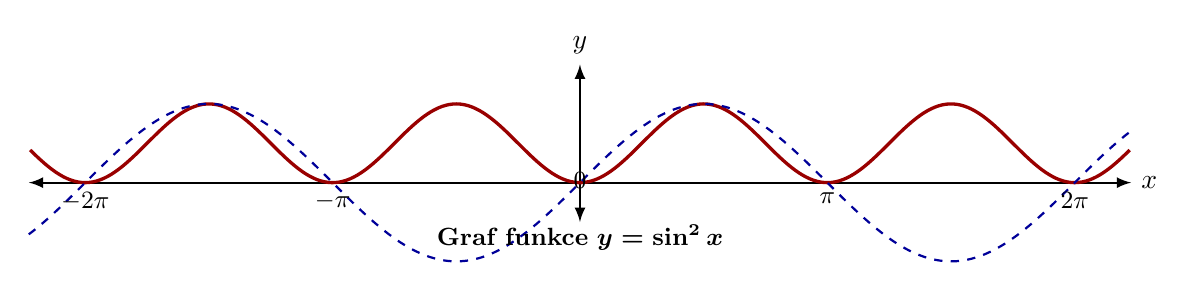
\begin{tikzpicture}[scale=1, >=latex]
            % ==== AXES ====
            \draw[<->, thick] (-7,0) -- (7,0) node[right] {$x$};
            \draw[<->, thick] (0,-0.5) -- (0,1.5) node[above] {$y$};
            % ==== SINUS^2 CURVE ====
            \draw[very thick, red!60!black, samples=300, domain=-2*pi-0.7:2*pi+0.7]
                plot(\x,{(sin(\x r))^2});
            \draw[thick, blue!60!black, dashed, samples=300, domain=-7:7]
                plot(\x,{sin(\x r)});
            \node[below] at (0,0.25) {\small $0$};
            \node[below] at ({-2*pi},0) {\small $-2\pi$};
            \node[below] at ({-pi},0) {\small $-\pi$};
            \node[below] at ({pi},0) {\small $\pi$};
            \node[below] at ({2*pi},0) {\small $2\pi$};
           
            % ==== Title ====
            \node at (0,-0.7) {\small \textbf{Graf funkce} $\boldsymbol{y = \sin^2 x}$};
         \end{tikzpicture}
    \end{center}
    V tomto grafu můžeme vidět, že všechny záporné hodnoty funkce sinus byly převedeny na kladné hodnoty,
    což vytváří charakteristický tvar vlny, která se dotýká osy $x$ v bodech, kde je sinus roven nule.
\end{examplebox}

Poslední příklad, který je dobré si ukázat je funkce s absolutní hodnotou.

\begin{examplebox}
    Mějme funkci:
    \[y = |\cos x|.\]
    Tento graf můžeme vytvořit tak, že nejprve nakreslíme základní graf funkce $y = \cos x$,
    a poté pro každé $x$ na ose $x$ vezmeme absolutní hodnotu hodnoty $y$.
    To znamená, že pokud je hodnota $y$ kladná, zůstane stejná, ale pokud je hodnota $y$ záporná, stane se kladnou.

    \textbf{1. Základní graf:}
    \begin{center}
        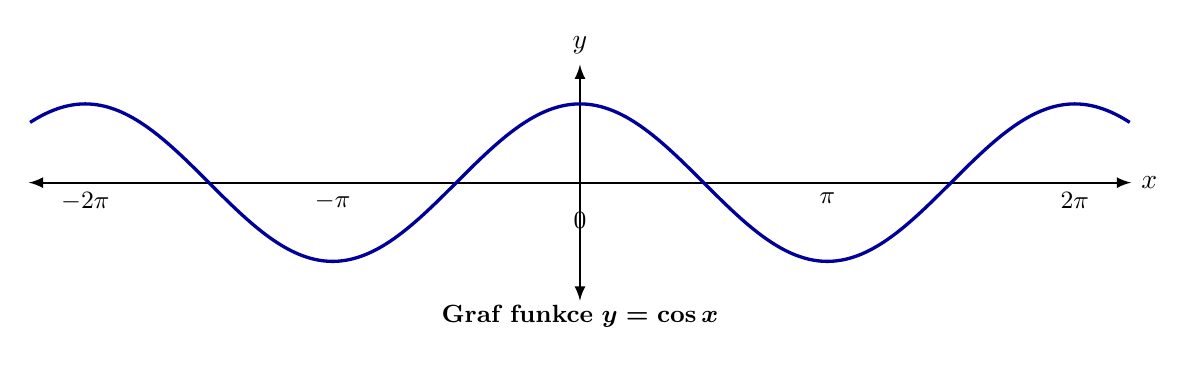
\begin{tikzpicture}[scale=1, >=latex]
            % ==== AXES ====
            \draw[<->, thick] (-7,0) -- (7,0) node[right] {$x$};
            \draw[<->, thick] (0,-1.5) -- (0,1.5) node[above] {$y$};
            % ==== COSINUS CURVE ====
            \draw[very thick, blue!60!black, samples=300, domain=-2*pi-0.7:2*pi+0.7]
                plot(\x,{cos(\x r)});
            \node[below] at (0,-0.25) {\small $0$};
            \node[below] at ({-2*pi},0) {\small $-2\pi$};
            \node[below] at ({-pi},0) {\small $-\pi$};
            \node[below] at ({pi},0) {\small $\pi$};
            \node[below] at ({2*pi},0) {\small $2\pi$};
           
            % ==== Title ====
            \node at (0,-1.7) {\small \textbf{Graf funkce} $\boldsymbol{y = \cos x}$};
         \end{tikzpicture}
    \end{center}

    \bigskip
    \textbf{2. Graf funkce} $\boldsymbol{y = |\cos x|}$:
    \begin{center}
        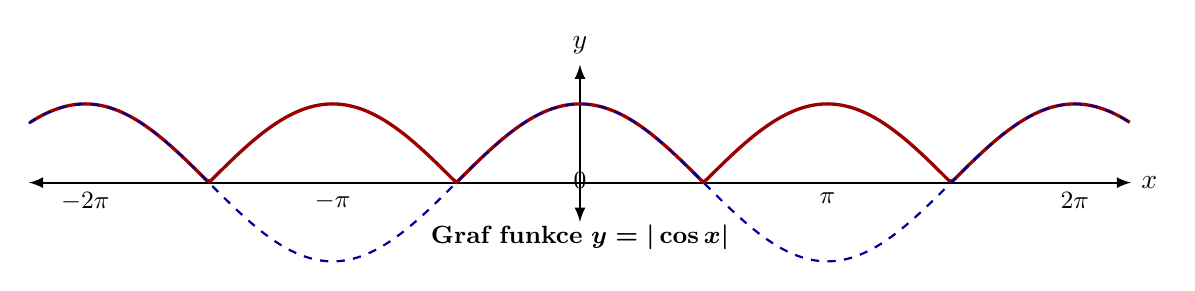
\begin{tikzpicture}[scale=1, >=latex]
            % ==== AXES ====
            \draw[<->, thick] (-7,0) -- (7,0) node[right] {$x$};
            \draw[<->, thick] (0,-0.5) -- (0,1.5) node[above] {$y$};
            % ==== ABSOLUTE COSINUS CURVE ====
            \draw[very thick, red!60!black, samples=300, domain=-2*pi-0.7:2*pi+0.7]
                plot(\x,{abs(cos(\x r))});
            \draw[thick, blue!60!black, dashed, samples=300, domain=-7:7]
                plot(\x,{cos(\x r)});
            \node[below] at (0,0.25) {\small $0$};
            \node[below] at ({-2*pi},0) {\small $-2\pi$};
            \node[below] at ({-pi},0) {\small $-\pi$};
            \node[below] at ({pi},0) {\small $\pi$};
            \node[below] at ({2*pi},0) {\small $2\pi$};

            % ==== Title ====
            \node at (0,-0.7) {\small \textbf{Graf funkce} $\boldsymbol{y = |\cos x|}$};
         \end{tikzpicture}
    \end{center}
    V tomto grafu můžeme vidět, že všechny záporné hodnoty funkce kosinus byly převedeny na kladné hodnoty,
    což vytváří charakteristický tvar vlny, která se dotýká osy $x$ v bodech, kde je kosinus roven nule.
\end{examplebox}


Stejnými způsoby můžeme vytvářet grafy i pro další goniometrické funkce, jako je právě sinus, kosinus, tangens nebo kotangens,
a také pro jejich různé úpravy a kombinace.

A když nyní umíme posuny a úpravy goniometrických funkcí. Můžeme si uázat proč platí vztah mezi sinus a kosinus:
\[\sin x = \cos\left(x - \frac{\pi}{2}\right).\]
Tento vztah totiž vyplývá z faktu, že kosinus je posunutý sinus o $\frac{\pi}{2}$ doleva.

\begin{center}
    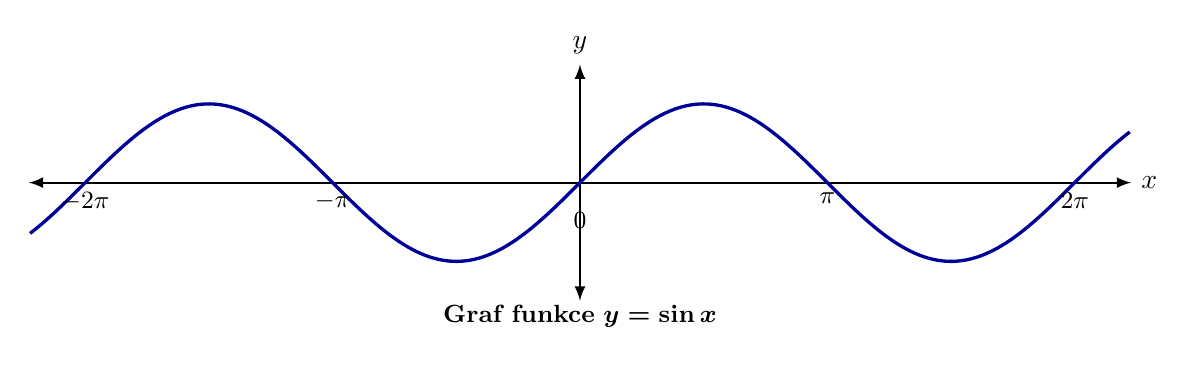
\begin{tikzpicture}[scale=1, >=latex]
        % ==== AXES ====
        \draw[<->, thick] (-7,0) -- (7,0) node[right] {$x$};
        \draw[<->, thick] (0,-1.5) -- (0,1.5) node[above] {$y$};
        % ==== SINUS CURVE ====
        \draw[very thick, blue!60!black, samples=300, domain=-2*pi-0.7:2*pi+0.7]
            plot(\x,{sin(\x r)});
        \node[below] at (0,-0.25) {\small $0$};
        \node[below] at ({-2*pi},0) {\small $-2\pi$};
        \node[below] at ({-pi},0) {\small $-\pi$};
        \node[below] at ({pi},0) {\small $\pi$};
        \node[below] at ({2*pi},0) {\small $2\pi$};
       
        % ==== Title ====
        \node at (0,-1.7) {\small \textbf{Graf funkce} $\boldsymbol{y = \sin x}$};
     \end{tikzpicture}

     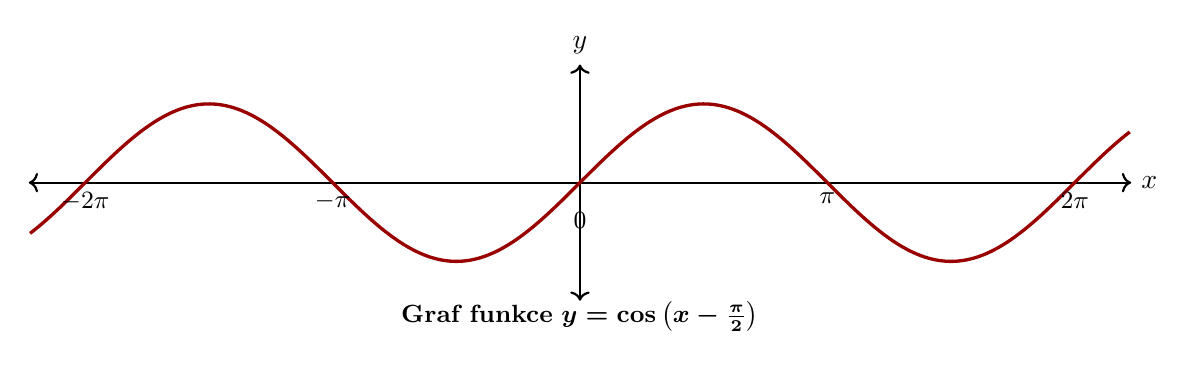
\begin{tikzpicture}
        % ==== AXES ====
        \draw[<->, thick] (-7,0) -- (7,0) node[right] {$x$};
        \draw[<->, thick] (0,-1.5) -- (0,1.5) node[above] {$y$};
        % ==== COSINE SHIFTED CURVE ====
        \draw[very thick, red!60!black, samples=300, domain=-2*pi-0.7:2*pi+0.7]
            plot(\x,{cos((\x - pi/2) r)});
        \node[below] at (0,-0.25) {\small $0$};
        \node[below] at ({-2*pi},0) {\small $-2\pi$};
        \node[below] at ({-pi},0) {\small $-\pi$};
        \node[below] at ({pi},0) {\small $\pi$};
        \node[below] at ({2*pi},0) {\small $2\pi$};
       
        % ==== Title ====
        \node at (0,-1.7) {\small \textbf{Graf funkce} $\boldsymbol{y = \cos\left(x - \frac{\pi}{2}\right)}$};
     \end{tikzpicture}
\end{center}
Jak vidíme, oba grafy jsou identické, což potvrzuje platnost tohoto vztahu mezi funkcemi sinus a kosinus:
\[
\sin x = \cos\left(x - \frac{\pi}{2}\right).
\]

Tento vztah můžeme zároveň odvodit z geometrického významu těchto funkcí na jednotkové kružnici, jak jsme si ukázali na začátku této kapitoly.
A to pomocí \important{součtových vzorců}, které si rozebereme v další kapitole.

\section{Cyklometrické funkce}

\important{Cyklometrické funkce} jsou \textbf{inverzní funkce} k základním \textbf{goniometrickým funkcím}.
To znamená, že pokud máme goniometrickou funkci, jako je například sinus, 
tak její inverzní funkce je \textbf{arkus sinus} (označována jako $\arcsin$ nebo $\sin^{-1}$).
Podobně inverzní funkcí k funkci kosinus je \textbf{arkus kosinus} ($\arccos$ nebo $\cos^{-1}$) 
a k funkci tangens je \textbf{arkus tangens} ($\arctan$ nebo $\tan^{-1}$).  

Tyto funkce nám umožňují najít úhel, pokud známe hodnotu goniometrické funkce.
Například, pokud víme, že $\sin \varphi = 0.5$, můžeme použít arkus sinus k nalezení úhlu $\varphi$:
\[\varphi = \arcsin(0.5) = \frac{\pi}{6}.\]

Cyklometrické funkce mají omezený definiční obor a obor hodnot, aby byly jednoznačné.
Například:
\begin{itemize}
    \item Definiční obor funkce \textbf{$\arcsin x$} je $\langle-1, 1\rangle$ a obor hodnot je $\langle-\frac{\pi}{2}, \frac{\pi}{2}\rangle$.
    \item Definiční obor funkce \textbf{$\arccos x$} je $\langle-1, 1\rangle$ a obor hodnot je $\langle0, \pi\rangle$.
    \item Definiční obor funkce \textbf{$\arctan x$} je $\mathbb{R}$ a obor hodnot je $\left(-\frac{\pi}{2}, \frac{\pi}{2}\right)$.
    \item Definiční obor funkce \textbf{$\arccot x$} je $\mathbb{R}$ a obor hodnot je $(0, \pi)$.
\end{itemize}

Tyto funkce jsou užitečné v mnoha oblastech matematiky, fyziky a inženýrství, kde je potřeba pracovat s úhly a jejich goniometrickými hodnotami.

Nyní si ukážeme dva grafy cyklometrických funkcí $\arcsin x$ a $\arccos x$ vedle sebe pro lepší porovnání.

\begin{center}
    \begin{tikzpicture}[scale=2, >=latex]
        % ==== AXES ====
        \draw[<->, thick] (-1.5,0) -- (1.5,0) node[right] {$x$};
        \draw[<->, thick] (0,-2) -- (0,2) node[above] {$y$};
        % ==== ARCSIN CURVE ====
        \draw[very thick, blue!60!black, samples=300, domain=-1.57:1.57]
            plot({sin(\x r)},\x);
        \node[below] at (0,-0.25) {\small $0$};
        \node[below] at (1,0) {\small $1$};
        \node[below] at (-1,0) {\small $-1$};
        \node[left] at (0,{pi/2}) {\small $\frac{\pi}{2}$};
        \node[left] at (0,{-pi/2}) {\small $-\frac{\pi}{2}$};

        % ==== Vertical and Horizontal Lines ====
        \draw[dashed] (1,0) -- (1,{pi/2});
        \draw[dashed] (-1,0) -- (-1,{-pi/2});
        \draw[dashed] (0,{pi/2}) -- (1,{pi/2});
        \draw[dashed] (0,{-pi/2}) -- (-1,{-pi/2});
       
        % ==== Title ====
        \node at (0,-2.3) {\small \textbf{Graf funkce} $\boldsymbol{y = \arcsin x}$};
     \end{tikzpicture}
     \hspace{2cm}
     \begin{tikzpicture}[scale=2, >=latex]
        % ==== AXES ====
        \draw[<->, thick] (-1.5,0) -- (1.5,0) node[right] {$x$};
        \draw[<->, thick] (0,-0.5) -- (0,3.5) node[above] {$y$};
        % ==== ARCCOS CURVE ====
        \draw[very thick, red!60!black, samples=300, domain=0:3.14]
            plot({cos(\x r)},\x);
        \node[right] at (0,1.57) {\small $\frac{\pi}{2}$};
        \node[below] at (1,0) {\small $1$};
        \node[below] at (-1,0) {\small $-1$};
        \node[right] at (0,3.14) {\small $\pi$};
        \node[below] at (0.2,0) {\small $0$};
        % ==== Vertical and Horizontal Lines ====
        \draw[dashed] (-1,0) -- (-1,3.14);
        \draw[dashed] (0,3.14) -- (-1,3.14);

        % ==== Title ====
        \node at (0,-0.7) {\small \textbf{Graf funkce} $\boldsymbol{y = \arccos x}$};
     \end{tikzpicture}
\end{center}

Pro tyto funkce platí následující vztahy:
\[\arcsin(\sin x) = x \quad \text{pro } x \in \left\langle -\frac{\pi}{2}, \frac{\pi}{2} \right\rangle,\]
\[\arccos(\cos x) = x \quad \text{pro } x \in \langle 0, \pi \rangle,\]

Stejně tak pro tangens a kotangens platí:
\[\arctan(\tan x) = x \quad \text{pro } x \in \left(-\frac{\pi}{2}, \frac{\pi}{2}\right),\]
\[\arccot(\cot x) = x \quad \text{pro } x \in (0, \pi).\]

\begin{notebox}
    \textbf{Poznámka:} Stejně jako jsme měli u kvadratických funkcí a rovnic pro hodnoty $x^2$ nebo obecně jakékoliv hodnoty $6^2 = 36$
    symbol pro inverzní funkci mocniny byla odmocnina, tak i zde máme speciální symboly pro inverzní funkce goniometrických funkcí a sice právě \textbf{Cyklometrické funkce ($\arcsin x, \arccos x, \arctan x, \arccot x$ )}.
    Protože goniometrické funkce nejsou jednoznačné na celém svém definičním oboru, musíme omezit jejich definiční obory, aby inverzní funkce byly jednoznačné.
    To znamená, že například pro funkci \textbf{$\sin x$} musíme omezit definiční obor na interval $\left\langle -\frac{\pi}{2}, \frac{\pi}{2} \right\rangle$,
    aby inverzní funkce \textbf{$\arcsin x$} byla jednoznačná.
\end{notebox}


% -----------------------------------------------------------------
% ---------------------- P Ř Í K L A D Y --------------------------
% -----------------------------------------------------------------

\exercisepart
\setcounter{section}{1}
% =========================
% ÚLOHA 1 – Nakreslte grafy funkcí
% =========================
\begin{exercise}[Nakreslete grafy funkcí]
    Nakreslete grafy následujících základních goniometrických funkcí:
    \begin{tasks}(2)
        \task $y = \sin x $
        \task $y = \cos x $
        \task $y = \tan x $
        \task $y = \cot x $
    \end{tasks}
\end{exercise}


% =========================
% ÚLOHA 2 – Převěď radiány na stupně
% =========================
\begin{exercise}[Převěď radiány na stupně]
    Převěďte následující úhly z radiánů na stupně:
    \begin{tasks}(4)
        \task $\frac{\pi}{6} $
        \task $-\frac{\pi}{4} $
        \task $\frac{\pi}{3} $
        \task $-\frac{\pi}{2} $
        \task $\pi $
        \task $-\frac{2\pi}{3} $ 
        \task $\frac{5\pi}{6} $
        \task $- \pi $
        \task $16\frac{\pi}{6} $
        \task $-10\frac{\pi}{4} $
        \task $8\frac{\pi}{3} $
        \task $-6\frac{\pi}{2} $
        \task $9\pi $
        \task $-7\frac{2\pi}{3} $
        \task $5\frac{5\pi}{6} $
        \task $-4\pi $
    \end{tasks}
\end{exercise}


% =========================
% ÚLOHA 3 – Převod mezi stupni a radiány
% =========================
\begin{exercise}[Převod mezi stupni a radiány]
Vypočítejte následující hodnoty:

\begin{tasks}(1)
    \task \textbf{Velikost jednoho stupně v radiánech.}
    \task \textbf{Velikost jednoho radiánu ve stupních.}
\end{tasks}

\end{exercise}


% =========================
% ÚLOHA 4 – Převěď stupně na radiány
% =========================
\begin{exercise}[Převěď stupně na radiány]
    Převěďte následující úhly ze stupňů na radiány:
    \begin{tasks}(4)
        \task $30^\circ $
        \task $-45^\circ $
        \task $60^\circ $
        \task $-90^\circ $
        \task $180^\circ $
        \task $-120^\circ $ 
        \task $150^\circ $
        \task $-180^\circ $
        \task $1550^\circ $
        
    \end{tasks}
\end{exercise}


% =========================
% ÚLOHA 5 – Najděte tabulkové hodnoty goniometrických funkcí
% =========================
\begin{exercise}[Najděte tabulkové hodnoty goniometrických funkcí]
    Najděte hodnoty následujících goniometrických funkcí pro dané úhly:
    \begin{tasks}(4)
        \task $\sin \frac{\pi}{6} $
        \task $\cos -\frac{\pi}{3} $
        \task $\tan \frac{\pi}{4} $
        \task $\cot \frac{\pi}{3} $
        \task $\sin -\frac{\pi}{2} $
        \task $\cos 0 $ 
        \task $\tan \frac{\pi}{2} $
        \task $\cot 0 $
        \task $\sin \pi $
        \task $\cos \pi $
        \task $\sin -\pi $
        \task $\cos -\frac{\pi}{2} $
        \task $\tan -\frac{\pi}{4} $
        \task $\cot -\frac{\pi}{3} $
        \task $\sin -\frac{3\pi}{2} $
        \task $\cos \frac{3\pi}{2} $
        \task $\tan \pi $
        \task $\cot \pi $
        \task $\sin \frac{2\pi}{3} $
        \task $\cos \frac{5\pi}{6} $
    \end{tasks}
\end{exercise}


% =========================
% ÚLOHA 6 – Najděte úhly tabulkových hodnot goniometrických funkcí
% =========================
\begin{exercise}[Najděte úhly tabulkových hodnot goniometrických funkcí]
    Najděte úhly pro následující hodnoty goniometrických funkcí:
    \begin{tasks}(4)
        \task $\arcsin \frac{1}{2} $
        \task $\arccos \frac{\sqrt{3}}{2} $
        \task $\arctan 1 $
        \task $\arccot \sqrt{3} $
        \task $\arcsin -1 $
        \task $\arccos 0 $ 
        \task $\arctan 0 $
        \task $\arccot -1 $
        \task $\arcsin 0 $
        \task $\arccos -1 $
        \task $\arcsin \frac{\sqrt{2}}{2} $
        \task $\arccos -\frac{\sqrt{2}}{2} $
        \task $\arctan -1 $
        \task $\arccot -\sqrt{3} $
        \task $\arcsin -\frac{\sqrt{3}}{2} $
        \task $\arccos -2 $
    \end{tasks}
\end{exercise}


% =========================
% ÚLOHA 7 – Najděte úhly tabulkových hodnot goniometrických funkcí
% =========================
\begin{exercise}[Najděte úhly tabulkových hodnot goniometrických funkcí]
    Najděte úhly pro následující hodnoty goniometrických funkcí:
    \begin{tasks}(4)
        \task $\sin x = \frac{1}{2} $
        \task $\cos x = -\frac{\sqrt{3}}{2} $
        \task $\tan x = \frac{\sqrt{3}}{3} $
        \task $\cot x = \sqrt{3} $
        \task $\sin x = -\frac{1}{2} $
        \task $\cos x = \frac{-\sqrt{2}}{2} $
        \task $\tan x = -1 $
        \task $\cot x = -\sqrt{3} $
        \task $\sin x = 0 $
        \task $\cos x = 0 $
        \task $\tan x = 1 $
        \task $\sin x = \frac{\sqrt{3}}{2} $
        \task $\cos x = \frac{1}{2} $
        \task $\cot x = 1 $
        \task $\sin x = -\frac{\sqrt{3}}{2} $
        \task $\cos x = -\frac{1}{2} $
    \end{tasks}
\end{exercise}


\setcounter{section}{2}
% =========================
% ÚLOHA 8 – Eiffelova věž
% =========================
\begin{exercise}[Výškový úhel – Eiffelova věž]
    Vrchol Eiffelovy věže je vidět ze vzdálenosti $500\,\text{m}$ pod výškovým úhlem 
    $32^\circ 57'$. Určete výšku Eiffelovy věže (zanedbejte nerovnost terénu).
\end{exercise}


% =========================
% ÚLOHA 9 – Šířka řeky
% =========================
\begin{exercise}[Šířka řeky]
    Na břehu řeky jsou dva stromy vzdálené od sebe $50\,\text{m}$. 
    Na protějším břehu stojí třetí strom tak, že spolu s předchozími tvoří pravoúhlý trojúhelník, 
    jehož jednou odvěsnou je šířka řeky a druhou odvěsnou úsek mezi stromy na břehu. 
    Určete šířku řeky, jestliže přepona tohoto „stromového“ trojúhelníku svírá s břehem úhel $67^\circ$.
\end{exercise}


% =========================
% ÚLOHA 10 – Určení velikostí úhlů v trojúhelníku
% =========================
\begin{exercise}[Určete velikosti úhlů v trojúhelníku]
Mějme pravoúhlý trojúhelník $ABC$ s vnitřními úhly $\alpha, \beta, \gamma$, kde
$\alpha = 90^\circ$, $\beta = 30^\circ$, $\gamma = 60^\circ$.
Určete velikosti následujících úhlů:
\begin{tasks}(2)
    \task $\angle ABC$
    \task $\angle ACB$
    \task $\angle CAB$
    \task $\angle CBA$
\end{tasks}
\end{exercise}


% =========================
% ÚLOHA 11 – Načrtněte úhly na jednotkové kružnici
% =========================
\begin{exercise}[Načrtněte úhly na jednotkové kružnici]
Načrtněte do jednotkové kružnice následující orientované úhly:
\begin{tasks}(3)
    \task $30^\circ$
    \task $70^\circ$
    \task $\frac{\pi}{2}$
    \task $200^\circ$
    \task $\frac{3\pi}{2}$
    \task $-\frac{12\pi}{5}$
    \task $315^\circ$
    \task $-\frac{\pi}{3}$
    \task $540^\circ$
\end{tasks}
\end{exercise}


% =========================
% ÚLOHA 12 - Vypočítej hodnoty goniometrických funkcí
% =========================
\begin{exercise}[Vypočítej hodnoty goniometrických funkcí]
Vypočítejte hodnoty následujících goniometrických funkcí pomocí tabulek anebo kalkulačky na 4 desetinná místa:
\begin{tasks}(4)
    \task $\sin 144^\circ21'$
    \task $\cos 225^\circ30'$
    \task $\sin 1$
    \task $\cos 5,4$
    \task $\sin(-150^\circ13')$
    \task $\sin 4,2$
    \task $\cos 3,14$
    \task $\sin 126^\circ47'$
\end{tasks}
\end{exercise} 


% =========================
% ÚLOHA 13 – Základní velikosti úhlů ve stupních
% =========================
\begin{exercise}[Základní velikosti úhlů ve stupních]
Napište velikosti následujících základních úhlů ve stupních:
\begin{tasks}(2)
    \task $\sin \alpha = \dfrac{\sqrt{3}}{2} \wedge \cos \alpha < 0$
    \task $\cos \beta = -\dfrac{1}{2} \wedge \sin \beta > 0$
    \task $\sin \gamma = -\dfrac{1}{2} \wedge \cos \gamma < 0$
    \task $\cos \delta = \dfrac{\sqrt{2}}{2} \wedge \sin \delta < 0$
    \task $\sin \epsilon = -\dfrac{1}{2}$
    \task $\cos \zeta = 2$
    \end{tasks}
\end{exercise}


% =========================
% ÚLOHA 14 – Nakreslte grafy funkcí sinus s úpravami
% =========================
\begin{exercise}[Nakreslete grafy funkcí s úpravami]
    Nakreslete grafy následujících funkce, určete periodu, vypočítejte průsečíky grafu s osou $x$ a i s osou $y$ a určete obor hodnot:
    \begin{tasks}(3)
        \task $y = \sin x $
        \task $y = \sin x + 2$
        \task $y = \sin (x + 2)$
        \task $y = 2 \sin x $
        \task $y = -\sin x $
        \task $y = -\sin x + 2$
        \task $y = -2 \sin(-x)$
        \task $y = \sin 2x$
        \task $y = \sin (-2x)$
        \task $y = \sin \dfrac{1}{2}x$
        \task $y = \sin \left(-\dfrac{1}{2}x\right)$
        \task $y = -\dfrac{1}{2} \sin \left(\dfrac{x}{2} - \dfrac{\pi}{4} \right)$
    \end{tasks}
\end{exercise}


% =========================
% ÚLOHA 15 – Nakreslete grafy funkcí kosinus s úpravami
% =========================
\begin{exercise}[Nakreslete grafy funkcí kosinus s úpravami]
    Nakreslete grafy následujících funkce, určete periodu, vypočítejte průsečíky grafu s osou $x$ a i s osou $y$ a určete obor hodnot:
    \begin{tasks}(3)
        \task $y = \cos x $
        \task $y = 2 \cos (-2x)$
        \task $y = \cos x - \dfrac{\pi}{4}$
        \task $y = \dfrac{\pi}{4} - \cos x$
        \task $y = \cos (x - \dfrac{\pi}{4})$
        \task $y = \dfrac{1}{2}\cos \left(x - \dfrac{\pi}{4}x\right)$
        \task $y = -\cos \left( \dfrac{\pi}{4} - x\right)$
        \task $y = \cos \left( \dfrac{x}{2} - \dfrac{\pi}{4}\right)$
        \task $y = -\dfrac{1}{2} \cos 4x$
        \task $y = \cos \dfrac{\pi}{4}x$
        \task $y = -\cos \dfrac{x}{2}$
        \task $y = -\dfrac{1}{2} \cos \left(\dfrac{x}{2} + \dfrac{\pi}{4} \right)$
    \end{tasks}
\end{exercise}


% =========================
% ÚLOHA 16 – Nakreslte grafy cyklometrických funkcí
% =========================
\begin{exercise}[Nakreslete grafy cyklometrických funkcí]
    Nakreslete grafy následujících cyklometrických funkcí:
    \begin{tasks}(2)
        \task $y = \arcsin x $
        \task $y = \arccos x $
        \task $y = \arctan x $
        \task $y = \arccot x $
    \end{tasks}
\end{exercise}


\newpage
% =========================
% ÚLOHA 17 – Nakreslete grafy cyklometrických funkcí s úpravami
% =========================
\begin{exercise}[Nakreslete grafy cyklometrických funkcí s úpravami]
    Nakreslete grafy následujících cyklometrických funkcí s úpravami:
    \begin{tasks}(2)
        \task $y = \arcsin (x - 0.5) $
        \task $y = \arccos (x + 0.5) $
        \task $y = \arctan x + 1 $
        \task $y = \arccot x - 1 $
        \task $y = 2 \arcsin x $
        \task $y = 0.5 \arccos x $ 
        \task $y = \arctan(3x - 1) + 2 $
        \task $y = \arccot(0.5x + 2) - 2 $
    \end{tasks}
\end{exercise}

% =========================
% ÚLOHA 18 – Načertněte grafy funkcí a porovnejte dvojice
% =========================
\begin{exercise}[Načrtněte grafy funkcí a porovnejte dvojice]
    Načrtněte grafy následujících funkcí $f_1$ až $f_6$, $g_1$ až $g_6$ a podle obrázku rozhodnětě, které dovjice funkcí se sobě rovnají:
    \begin{tasks}(2)
        \task $f_1(x) = \sin x $
        \task $f_2(x) = \cos\left(x - \dfrac{\pi}{2}\right) $
        \task $f_3(x) = -\sin(-x) $
        \task $f_4(x) = \cos\left(-x + \dfrac{\pi}{2}\right) $
        \task $f_5(x) = \sin\left(x + 2\pi\right) $
        \task $f_6(x) = \cos\left(x - \dfrac{5\pi}{2}\right) $
        \task $g_1(x) = \cos x $
        \task $g_2(x) = \sin\left(x + \dfrac{\pi}{2}\right) $
        \task $g_3(x) = -\cos(-x) $
        \task $g_4(x) = \sin\left(-x - \dfrac{\pi}{2}\right) $
        \task $g_5(x) = \cos\left(x + 2\pi\right) $
        \task $g_6(x) = \sin\left(x + \dfrac{5\pi}{2}\right) $
    \end{tasks}
\end{exercise}

% =========================
% ÚLOHA 19 – Načrtněte grafy funkcí
% =========================
\begin{exercise}[Načrtněte grafy funkcí]
    Načrtněte grafy funkcí a určete definiční obor, obor hodnot, periodu a vypočíteje průsečíky s osou $x$ a $y$:
    \begin{tasks}(2)
        \task $f_1(x) = \cot x$
        \task $f_2(x) = \cot x - \dfrac{\pi}{3}$
        \task $f_3(x) = \dfrac{\pi}{3} - \cot x$
        \task $f_4(x) = -\cot(-x)$
        \task $f_5(x) = \frac{1}{2} \cot \left(x - \dfrac{\pi}{4}\right)$
        \task $f_6(x) = \cot \left(\dfrac{x}{2} - \dfrac{\pi}{3}\right)$
        \task $f_7(x) = -\dfrac{1}{2} \cot 2x$
        \task $f_8(x) = \cot x\pi$
        \task $f_9(x) = \cot \left(\frac{\pi}{3} - x\right)$
        \task $f_{10}(x) = -\cot \dfrac{x}{2}$
    \end{tasks}
\end{exercise}


% =========================
% ÚLOHA 20 - Načrtněte grafy funkci
% =========================
\begin{exercise}[Načrtněte grafy funkcí]
    Načrtněte grafy funkcí v intervalu $\left(0; 2\pi\right)$:
    \begin{tasks}(2)
        \task $y = \sin^2 x$
        \task $y = \cos^2 x$
        \task $y = \sin x + \cos x$
        \task $y = \sin x - \cos x$
        \task $y = \sin^{-1} x$
        \task $y = \cos^{-1} x$
        \task $y = \sin^2 x + \cos^2 x$
        \task $y = \sin^2 x - \cos^2 x$
    \end{tasks}
\end{exercise}


\setcounter{section}{3}
% =========================
% ÚLOHA 21 - Grafy goniometrických funkcí sin s absolutní hodnotou
% =========================
\begin{exercise}[Načrtněte grafy funkcí]
    Načrtněte grafy funkcí:
    \begin{tasks}(2)
        \task $y = \left|\sin x \right|$
        \task $y = \left|\sin x \right| - \dfrac{1}{2}$
        \task $y = \left|\sin x - \dfrac{1}{2} \right|$
        \task $y = \sin \left|x\right|$
        \task $y = \sin \left|x + \dfrac{\pi}{6}\right|$
        \task $y = \sin\left(\left|x\right| + \dfrac{\pi}{6}\right)$
        \task $y = 1 - \left|\sin x \right|$
        \task $y = \left|2 \sin x - 1\right|$
        \task $y = 2 \left|\sin x\right| - 1$
        \task $y = \left|\sin x + \dfrac{\pi}{4}\right|$
    \end{tasks}
\end{exercise}


% =========================
% ÚLOHA 22 - Grafy goniometrických funkcí cos s absolutní hodnotou
% =========================
\begin{exercise}[Načrtněte grafy funkcí]
    Načrtněte grafy funkcí:
    \begin{tasks}(2)
        \task $y = \left|\cos x \right|$
        \task $y = \left|\cos x \right| + 1 $
        \task $y = \left|1 - \cos x \right| $
        \task $y = \left|1 - 2\cos x \right| $
        \task $y = \left|\left|\cos x \right| - \dfrac{1}{2}\right| $
        \task $y = \cos \left|x\right| $
        \task $y = \left|\cos x \right|+ \dfrac{\pi}{4} $
        \task $y = \left|\cos x + \dfrac{\pi}{4}\right| $
        \task $y = 2 \cos \left|x - \dfrac{\pi}{4}\right| $
        \task $y = \cos \left|x + \dfrac{\pi}{4}\right| - 2 $
    \end{tasks}
\end{exercise}


% =========================
% ÚLOHA 23 - Grafy goniometrických funkcí sin a cos
% =========================
\begin{exercise}[Načrtněte grafy funkcí]
    Načrtněte grafy funkcí:
    \begin{tasks}(3)
        \task $f_1: y = \sin x + \left| \sin x \right|$
        \task $f_2: y = \cos x - \left| \cos x \right|$
        \task $f_3: y = 2 \left| \sin x \right| \cos x$
        \task $f_4: y = -2\left| \cos x \sin x \right|$
        \task $f_5: y = \sin x \left| \cos x \right|$
        \task $f_6: y = \cos x \left| \sin x \right|$
        \task $f_7: y = \tan x \left| \cos x \right|$
        \task $f_8: y = \cot x \left| \sin x \right|$
    \end{tasks}
\end{exercise}


% =========================
% ÚLOHA 24 - Grafy goniometrických funkcí sin a cos v podílu
% =========================
\begin{exercise}[Načrtněte grafy funkcí]
    Načrtněte grafy funkcí:
    \begin{tasks}(2)
        \task $f_1: y = \dfrac{\sin x}{\left| \cos x \right|}$
        \task $f_2: y = \dfrac{\cos x}{\left| \sin x \right|}$
        \task $f_3: y = \dfrac{\left| \sin x \right|}{\cos x}$
        \task $f_4: y = \dfrac{\left| \cos x \right|}{\sin x}$
        \task $f_5: y = \dfrac{\sin x + \left| \sin x \right|}{\cos x - \left| \cos x \right|}$
        \task $f_6: y = \dfrac{\cos x + \left| \cos x \right|}{\sin x - \left| \sin x \right|}$
        \task $f_7: y = \dfrac{\sin x - \left| \cos x \right|}{\cos x + \left| \sin x \right|}$
        \task $f_8: y = \dfrac{\cos x - \left| \sin x \right|}{\sin x + \left| \cos x \right|}$
    \end{tasks}
\end{exercise}


\setcounter{section}{3}
% =========================
% ÚLOHA 18 – BONUS: Lichost tangensu
% =========================
\begin{exercise}[BONUS: Dokažte, že je tangens lichá funkce]
Dokažte, že funkce tangens je lichá, tedy že pro všechna $x$ z definičního oboru platí
\[
\tan(-x) = -\tan(x).
\]

\noindent
\textit{Nápověda:} Využijte vztah $\displaystyle \tan x = \frac{\sin x}{\cos x}$ a vlastnosti funkcí $\sin x$ a $\cos x$.
\end{exercise}



\end{document}